% =============================================================================
% Do We Still Need Fine-Tuning for Clinical Text Classification?
% Training-free semantic search vs. fine-tuned transformers (BPD screening)
% =============================================================================
\documentclass[11pt]{article}

\usepackage{graphicx}
\usepackage{authblk}
\usepackage[margin=1in]{geometry}
\usepackage[font=small,skip=4pt]{caption}
\usepackage{float}
\usepackage{microtype}
\usepackage[hyphens]{url}
\usepackage{booktabs}
\usepackage{multirow}
\usepackage{array}
\usepackage{makecell}
\usepackage{xcolor}
\usepackage{amsmath}
\usepackage{amssymb}
\usepackage{enumitem}
\usepackage{tikz}
\usetikzlibrary{shapes.geometric,arrows.meta,positioning,calc,fit,backgrounds}

\usepackage[backend=biber,style=numeric,sorting=none]{biblatex}
\addbibresource{references.bib}
\providecommand{\citealp}[1]{\cite{#1}}

\usepackage{hyperref}
\hypersetup{colorlinks=true,linkcolor=blue!60!black,citecolor=blue!60!black,urlcolor=blue!60!black}

\newcommand{\vbri}{VBRI}
\newcommand{\bpdqac}{BPDQAC}
\newcommand{\dsmv}{DSM-5}
\definecolor{ftblue}{HTML}{2A78D6}
\definecolor{vborange}{HTML}{EB6834}

\title{\textbf{Do We Still Need Fine-Tuning for Clinical Text Classification?
}}

\author[1]{Mehedi Hasan Moon\thanks{mehedi.hasan.moon@ict.mist.ac.bd}}
\author[1]{Md.\ Mahbubur Rahman}
\affil[1]{Department of Computer Science and Engineering, Military Institute of Science and Technology,
Mirpur Cantonment, Dhaka 1216, Bangladesh}
\date{\today}

\begin{document}
\maketitle

% =============================================================================
% ABSTRACT
% =============================================================================
\begin{abstract}
Fine-tuning a pretrained language model is now the usual way to build a text classifier. It needs
GPU training and a new set of weights for every task. This limits its use in low-resource clinical
settings. We ask a simple question: for a classification task, do we really need to fine-tune a
model, or can a frozen embedding model with semantic search do the job? We test this on borderline
personality disorder (BPD) screening with \bpdqac{}, a dataset of 3,258 expert-annotated
question--answer pairs from 362 participants who answered nine open-ended questions based on the
\dsmv{} Criterion A symptoms. We compare seven fine-tuned encoders (67M to 184M parameters), each
trained with three random seeds, with a training-free method that we call Vector-Based Retrieval
Inference (\vbri{}). \vbri{} encodes labelled answers once with a frozen embedding model
(\texttt{bge-base-en-v1.5}), keeps them in nine criterion-specific, class-balanced vector
databases, and labels a new answer by similarity-weighted $k$-nearest-neighbour voting. All settings
are chosen on a validation set. On 333 held-out answers, the best fine-tuned models reach about
84\% accuracy (ELECTRA 83.88\%, ModernBERT 84.78\%; means over three seeds). \vbri{} reaches only
70.57\% accuracy, so fine-tuning is clearly more accurate. Its BPD sensitivity is 80.60\%, which
lies inside the range of the fine-tuned means (77.61\% to 85.07\%). \vbri{} needs no training. It
builds its index in 9.6 seconds, against 2 to 13 minutes of GPU training, and stores 12.5\,MB for
the task, against 268 to 738\,MB for a fine-tuned model (the frozen encoder, shared across tasks,
is not counted). It also shows the stored answers behind every decision. Compared with a single
pooled index, isolating and balancing the criteria mainly raises BPD sensitivity; the effect on
accuracy is small. Semantic search is therefore not a replacement for fine-tuning. It is a cheap and
transparent option when quick updates, evidence for each decision and sensitivity matter more than
overall accuracy.
\end{abstract}

\noindent\textbf{Keywords:} text classification, sentence embeddings, semantic search, vector
database, $k$-nearest neighbours, training-free inference, fine-tuning, large language models,
borderline personality disorder, clinical NLP, resource-constrained deployment.

% =============================================================================
% 1. INTRODUCTION
% =============================================================================
\section{Introduction}\label{sec:intro}

Text classification is a core task in natural language processing (NLP). In health care, it helps
to sort patient messages, flag risk in clinical notes and screen people for mental health problems.
One recipe now dominates. Take a pretrained transformer such as BERT~\cite{devlin2019bert}. Then
fine-tune all of its weights on labelled examples. More recently, large language models (LLMs) have
joined in. They are prompted directly, or fine-tuned, for mental health
prediction~\cite{yang2024mentallama,xu2024mental,guo2024llmreview}. Behind all of this sits one
assumption: a classifier must be \emph{trained} for every new task.

This assumption has a cost. Fine-tuning needs a GPU and many hours of trial and error. Class
imbalance and overfitting must be handled with care. Every task gives a new set of weights. These
must be stored, versioned and retrained when the labels or the data change. The energy and money
cost of training is a known concern in NLP~\cite{strubell2019energy,schwartz2020green}. LLMs make
it worse. They have billions of parameters and often run on remote servers. They also raise privacy
questions when the input is clinical text~\cite{guo2024llmreview}. And they do not clearly win.
Several studies show that small fine-tuned encoders still beat zero-shot and few-shot LLMs on text
classification~\cite{bucher2024finetuned,edwards2024icl}. In mental health, zero-shot ChatGPT did
poorly on suicidality detection~\cite{lamichhane2023chatgpt}.

There is a third option, and it is often missed. Sentence embedding models turn text into dense
vectors. Texts with similar meaning land close together~\cite{reimers2019sbert,xiao2023cpack,muennighoff2023mteb}.
This is the idea behind semantic search and retrieval-augmented generation
(RAG)~\cite{karpukhin2020dpr,lewis2020rag}. Now think of a new patient answer. If it sits close to
many earlier answers that experts marked as BPD-indicative, we can give it the same label. No
gradient update is needed. The ``model'' is a frozen encoder plus a small database of labelled
vectors. We can update it by adding rows. It runs on modest hardware. Each decision can be explained
by showing the stored answers behind it. A recent clinical study found that text embeddings with a
light classifier detected depression in patient narratives better than GPT-4o~\cite{lho2025jama}.

The setting of this study makes these points important. Borderline personality disorder is a severe
condition. It shows as unstable relationships, unstable self-image and unstable emotions, together
with impulsive behaviour~\cite{dsm}. The median prevalence in the general population is about 1.6\%.
It rises to around 10\% in outpatient clinics and 20\% in psychiatric inpatients~\cite{dsm}. Between
40\% and 85\% of people with BPD attempt suicide, and up to 10\% die by
suicide~\cite{paris2001,stone1990,oumaya2008}. Diagnosis usually needs an interview with a licensed
clinician and tools such as the MSI-BPD~\cite{zanarini2003}. Access is a problem. In Bangladesh,
about 90\% of people with a mental health condition do not get treatment~\cite{huque2025}. A
screening tool for this setting must be cheap to build and run. It must be easy to update. It must
be clear to clinicians. And it should run locally, so that sensitive answers never leave the clinic.

So we ask a direct question. \textbf{Do we really need to fine-tune a language model to classify
clinical text, or can semantic search over a frozen embedding model do the job?} We answer it on
\bpdqac{}, a dataset of expert-labelled answers to structured BPD interview questions. We run a
controlled, head-to-head test of two paradigms. Both use the same data and the same test set.
Paradigm A is a set of fine-tuned transformer encoders. Paradigm B is a training-free retrieval
classifier that we call Vector-Based Retrieval Inference (\vbri{}).

The objectives of this work are:
\begin{enumerate}[leftmargin=*,itemsep=2pt]
  \item To compare fine-tuned encoders with retrieval methods on the same held-out clinical answers
        in terms of effectiveness, training time, inference time and storage.
  \item To develop \vbri{}, a training-free classifier that uses a frozen embedding model and nine
        criterion-isolated, class-balanced vector databases.
  \item To analyse cross-criterion contamination in a pooled index and to test, through an ablation,
        what criterion isolation and class balancing change.
  \item To assess the trade-off between fine-tuning and \vbri{} in accuracy, cost, ease of update
        and explainability.
\end{enumerate}

The paper is organised as follows. Section~\ref{sec:lit} reviews related work and states the
research gap. Section~\ref{sec:dataset} describes the dataset. Section~\ref{sec:method} explains
both methods and the reasons behind each decision. Section~\ref{sec:results} gives the results.
Section~\ref{sec:discussion} discusses what they mean and where they stop. Section~\ref{sec:conclusion}
concludes.

% =============================================================================
% 2. LITERATURE REVIEW
% =============================================================================
\section{Literature Review}\label{sec:lit}

This section follows the path that leads to our question. First, we show how mental health text
classification came to rely on trained and fine-tuned models. Then we look at what LLMs add, and
what they cost. Last, we review the embedding and retrieval methods that make a training-free
option possible.

\subsection{Mental health text classification: from feature engineering to fine-tuning}

Early work detected psychological states from social media posts with classical classifiers. Singh
et al.~\cite{singh2020framework} used NLP preprocessing with Logistic Regression, Support Vector
Machines, Na\"{i}ve Bayes and Decision Trees to detect antisocial behaviour on Twitter. A review by
Harrigian et al.~\cite{harrigian2021state} listed 102 social media mental health datasets. Most came
from Twitter and Reddit. Most studied depression and suicidal ideation. Most used self-reported
labels. These models relied on hand-made features. They struggled with subtle language.

Transformers changed this. Dinu and Moldovan~\cite{dinu2021automatic} fine-tuned BERT, RoBERTa and
XLNet on general Reddit posts and reached up to 81\% accuracy. Jiang et
al.~\cite{jiang-etal-2020-detection} used contextual BERT representations on 17.5 million posts
from users with eight disorders. Haque et al.~\cite{suicidalideationtransformers2020} reported
95.21\% accuracy with RoBERTa for suicidal ideation. Domain-adapted models followed. PsychBERT was
pretrained on mental health literature and social media~\cite{vajre2021psychbert}. MentalBERT and
MentalRoBERTa were pretrained on mental health subreddits~\cite{ji2022mentalbert}. BERT-based models
were also used for early self-harm detection~\cite{martinez2022early}. Reviews of this period agree
on two points~\cite{zhang2022natural,montejo2024survey,greco2023transformer}. Transformers dominate.
And most are trained on social media data with weak labels and little clinical validation. In every
case, a new task meant a new round of training.

\subsection{Personality disorder and BPD detection}

Work on personality disorders follows the same pattern. Jain et al.~\cite{jain2024} fine-tuned BERT
to classify four personality disorders and reached 74.7\% accuracy. Ellouze and
Belguith~\cite{ellouze2022hybrid,ellouze2022deep} combined CNN, BiLSTM and SVM layers to detect
personality disorders from tweets (F1 of 84\%). They later reviewed the move from classical to deep
models~\cite{ellouze2024artificial}. Baqasah et al.~\cite{baqasah2024personality} trained LSTMs on
social media text and reached 89\% accuracy.

Studies on BPD itself are rare. MindTime analysed diary entries with SVM and LSTM classifiers and
reached about 90\% accuracy~\cite{khazbak2021mindtime}. Wang et al.~\cite{wang2020learning} used
language and speech features from 50 non-clinical interviews to separate BPD, bipolar disorder and
healthy controls (AUROC 0.733). None of these studies used answers to structured diagnostic
questions. All of them trained a model for the task.

\subsection{Large language models for mental health: power and price}

LLMs promised to remove task-specific training. MentaLLaMA~\cite{yang2024mentallama} was
instruction-tuned on 105,000 samples. It gives predictions with explanations. Mental-LLM~\cite{xu2024mental}
showed that instruction fine-tuning improves LLMs a lot on mental health prediction. A systematic
review~\cite{guo2024llmreview} found promising results. It also found unstable outputs,
hallucinations, weak privacy control and ethical risks.

On classification itself, the evidence is mixed. Zero-shot ChatGPT reached an F1 of only 0.37 on
suicidality detection~\cite{lamichhane2023chatgpt}. Across many general benchmarks, fine-tuned
``small'' models such as RoBERTa still beat zero-shot GPT-3.5, GPT-4 and Claude
Opus~\cite{bucher2024finetuned}. Fine-tuning a smaller model also beats few-shot prompting of a
larger one~\cite{edwards2024icl}. So LLMs have not removed the need for training. They usually
add the fine-tuning of an even bigger model. Parameter-efficient methods such as
LoRA~\cite{hu2022lora} make this cheaper, but they do not make it go away.

\subsection{Embedding models, semantic search and training-free classification}

A separate line of work produced embedding models that are useful without task-specific training.
Sentence-BERT~\cite{reimers2019sbert} made it practical to compare sentences with cosine similarity.
Later models such as BGE~\cite{xiao2023cpack} learned from large and varied sets of text pairs.
The Massive Text Embedding Benchmark (MTEB)~\cite{muennighoff2023mteb} tests such models on
retrieval, clustering and classification. For classification, it trains a simple classifier on top
of frozen embeddings. Dense retrieval~\cite{karpukhin2020dpr}, fast similarity search with
FAISS~\cite{johnson2019faiss} and retrieval-augmented generation~\cite{lewis2020rag} made vector
databases a standard part of NLP systems.

Nearest-neighbour ideas also have a long history. $k$NN-LM showed that stored neighbours improve
language modelling~\cite{khandelwal2020knnlm}. Deep $k$-Nearest Neighbours used neighbours to make
predictions easier to interpret~\cite{papernot2018dknn}. Li et al.~\cite{li2023revisitknn} showed
that $k$NN improves and calibrates fine-tuned language models. SetFit~\cite{tunstall2022setfit}
reaches strong few-shot results by adapting a sentence encoder with contrastive learning. But it
still trains the encoder and a classification head.

In mental health, nearest-neighbour retrieval over message embeddings has been used for suicide
risk prediction on social media~\cite{fabregat2022clpsych}. Text embeddings with a light classifier
beat GPT-4o for depression detection from patient narratives~\cite{lho2025jama}.

Embeddings also have a known weakness. Sentence encoders often give a sentence and its negation a
very high similarity~\cite{chiang2023heros,cao2025negation}. This matters in clinical screening.
``I have never tried to hurt myself'' and ``I tried to hurt myself'' must not be treated as the same.
Any embedding-based screening tool must be built and checked with this in mind.

\subsection{Research gap and research questions}

Table~\ref{tab:gap} sums up the most relevant work. Three gaps stand out. First, almost all mental
health and BPD classifiers are trained or fine-tuned for their task. The few retrieval-based
systems use social media posts, not structured clinical answers. Second, studies rarely report
effectiveness and computing cost side by side on the same data. So the price of fine-tuning stays
hidden. Third, nobody has looked at why semantic search works or fails on structured interview data,
where several questions share the same emotional words. These gaps leave one basic question open:
\emph{do we really need to fine-tune a language model for a clinical classification task?}

\begin{table}[H]
\centering
\caption{Positioning of this work against representative prior studies.}
\label{tab:gap}
\small
\setlength{\tabcolsep}{4pt}
\resizebox{\textwidth}{!}{%
\begin{tabular}{@{}lllccc@{}}
\toprule
\textbf{Study} & \textbf{Data} & \textbf{Approach} & \makecell{\textbf{Task-specific}\\\textbf{training}} &
\makecell{\textbf{Cost}\\\textbf{reported}} & \makecell{\textbf{Built-in}\\\textbf{evidence}} \\
\midrule
Dinu \& Moldovan~\cite{dinu2021automatic} & Reddit & Fine-tuned BERT/RoBERTa/XLNet & Yes & No & No \\
Ji et al.~\cite{ji2022mentalbert} & Reddit & Domain-pretrained BERT & Yes & No & No \\
Jain et al.~\cite{jain2024} & PD-TXT & Fine-tuned BERT & Yes & No & No \\
Khazbak et al.~\cite{khazbak2021mindtime} & Diaries & SVM / LSTM & Yes & No & No \\
Wang et al.~\cite{wang2020learning} & 50 interviews & Speech + language features & Yes & No & No \\
Yang et al.~\cite{yang2024mentallama} & Social media & Instruction-tuned LLM & Yes & No & Text rationale \\
Lamichhane~\cite{lamichhane2023chatgpt} & Social media & Zero-shot ChatGPT & No & No & No \\
Fabregat et al.~\cite{fabregat2022clpsych} & Social media & ANN retrieval + RNN & Partly & No & No \\
Lho et al.~\cite{lho2025jama} & Patient narratives & Embeddings + XGBoost vs.\ LLM & Yes (head) & No & No \\
\midrule
\textbf{This work} & \textbf{Structured BPD interviews} & \textbf{Frozen embeddings + $k$NN (\vbri{})}
  & \textbf{No} & \textbf{Yes} & \textbf{Retrieved precedents} \\
\bottomrule
\end{tabular}}
\end{table}

We address the gap with three research questions.
\begin{description}[leftmargin=1.2cm,style=nextline,itemsep=2pt]
  \item[RQ1] Can a training-free semantic search classifier reach the BPD sensitivity of fine-tuned
             transformer encoders on structured clinical interview answers?
  \item[RQ2] What does each paradigm cost in training time, inference time and storage? What does
             the training-free approach give up in return?
  \item[RQ3] Which design decisions make semantic search work for criterion-structured clinical
             data?
\end{description}

We use fine-tuned encoders (67M to 184M parameters) as the comparison point. The literature above
shows that they are still the strongest practical classifiers. They usually match or beat prompted
LLMs on classification. If a training-free method can come close to them, it is a fair candidate
to replace the fine-tuning of larger models too.

% =============================================================================
% 3. DATASET
% =============================================================================
\section{The BPDQAC Dataset}\label{sec:dataset}

\bpdqac{} was built for BPD screening from structured interview answers. The interview has 14
questions. We wrote them with guidance from the \dsmv{}~\cite{dsm} and with help from psychologists
and psychiatrists. Nine open-ended questions cover the nine Criterion A symptoms: abandonment
avoidance, unstable relationships, identity disturbance, impulsive behaviour, suicidal and
self-harm behaviour, affective instability, chronic emptiness, inappropriate anger, and paranoid
ideation or dissociation. Five yes/no questions cover the general personality disorder Criteria B
to F. This study uses only the nine open-ended answers.

In total, 362 participants gave consent and completed the interview. This gave 3,258
question--answer pairs. An expert panel assessed each pair. The panel had a licensed psychiatrist, a
clinical psychologist and a trained counsellor. Each pair got one of three labels. \emph{Normal}
means no clinical symptom. \emph{BPD-indicative} means a pathological symptom that fits the \dsmv{}
severity level. \emph{Inconclusive} means mild distress, or too little information to decide.
Semi-supervised label propagation spread the expert labels across the full dataset.

The data are imbalanced (Figure~\ref{fig:data}a). There are 2,195 Normal, 673 BPD and 390
Inconclusive answers. The label mix also changes from question to question
(Figure~\ref{fig:data}b). Abandonment (Q1) and anger (Q8) give the most BPD answers. The suicidal
and self-harm question (Q5) gives the fewest. Later we show that this per-question imbalance is one
of the main reasons why a naive retrieval classifier fails.

\begin{figure}[H]
\centering
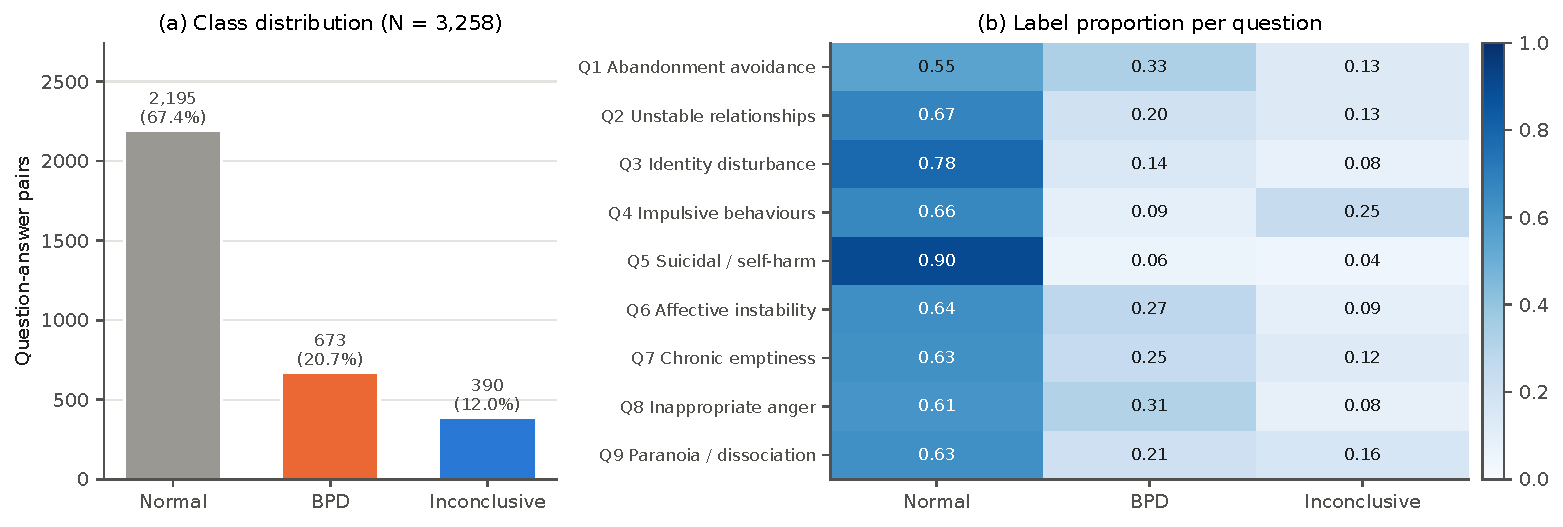
\includegraphics[width=\textwidth]{figures/generated/fig_data_overview.pdf}
\caption{Label structure of \bpdqac{} (3,258 original answers). (a) Overall class distribution.
(b) Label proportions per question.}
\label{fig:data}
\end{figure}

\paragraph{Splits and the training set.}
We split the data into training (2,592 answers), validation (333) and test (333) sets. The
validation and test sets are the same for both paradigms. We never augmented them. The test set has
225 Normal, 67 BPD and 41 Inconclusive answers, 37 per question.

The original training split is imbalanced (1,746 Normal, 538 BPD and 308 Inconclusive). Both
paradigms therefore use the same \emph{balanced} training set of 4,050 answers
(Figure~\ref{fig:aug}a). It holds exactly 150 Normal, 150 BPD and 150 Inconclusive answers for each
of the nine questions. We sub-sampled Normal answers and filled the minority classes with augmented
answers. Of the 4,050 answers, 2,250 are original and 1,800 are augmented (651 back-translation,
633 paraphrase, 516 synonym substitution). So about two thirds of the BPD and Inconclusive training
answers are augmented text (Figure~\ref{fig:aug}b). A second set of 4,279 answers, augmented but
not balanced per question (1,746 Normal, 1,612 BPD, 921 Inconclusive), is used only in the ablation.

No augmented text was made from a validation or test answer. A few very short, generic answers
(such as ``nothing significant'') appear in both the training and test sets. There are five such
texts, found in 14 training rows.

\begin{figure}[H]
\centering
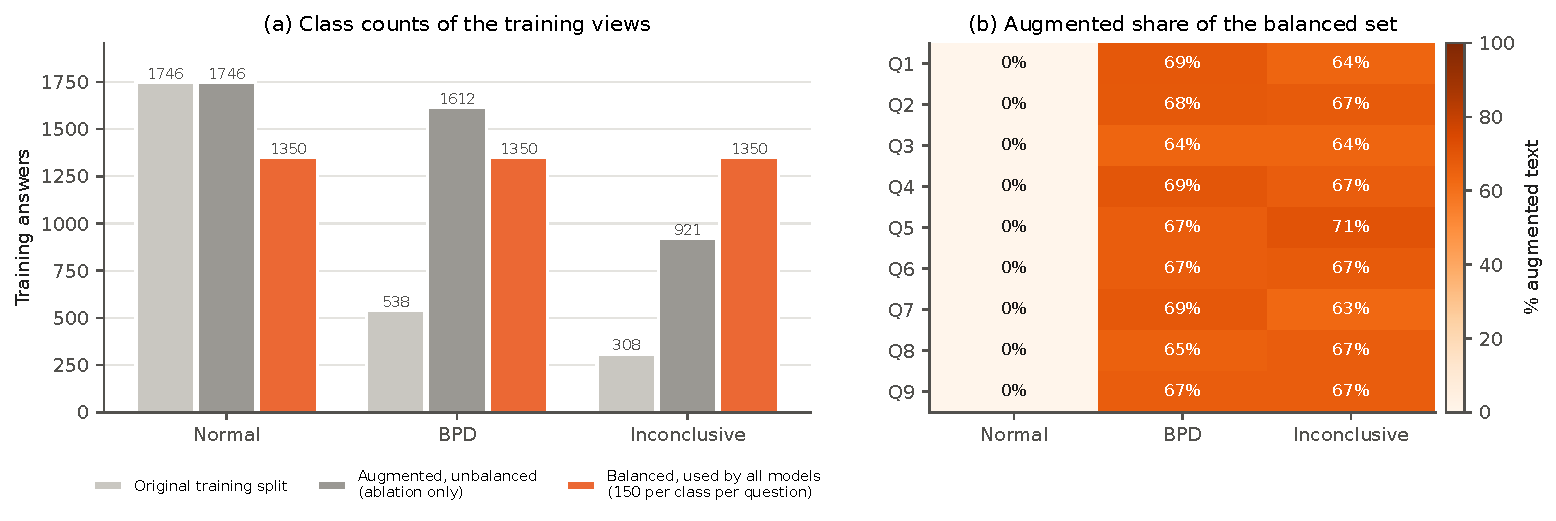
\includegraphics[width=\textwidth]{figures/generated/fig_training_views.pdf}
\caption{Training data. (a) Class counts of the original split, the unbalanced augmented set (used
only in the ablation) and the balanced set used by all models. (b) Share of augmented text in the
balanced set, per question and class.}
\label{fig:aug}
\end{figure}

% =============================================================================
% 4. METHODOLOGY
% =============================================================================
\section{Methodology}\label{sec:method}

We compare two ways of building the same three-class classifier (Normal, BPD, Inconclusive). Both
get the same input: a participant's answer to one of the nine questions. Both are scored on the same
333 test answers. Figure~\ref{fig:design} shows the overall study design.

% TODO(figure): study_design.pdf still shows old values (5,238 training answers, 3--18 min,
% 264--596 MB, 12 s, 12.4 MB, "BP DQAC"). Correct values: 4,050 balanced answers for both paradigms,
% 2--13 min, 268--738 MB, 9.6 s, 12.5 MB, "BPDQAC".
\begin{figure}[H]
\centering
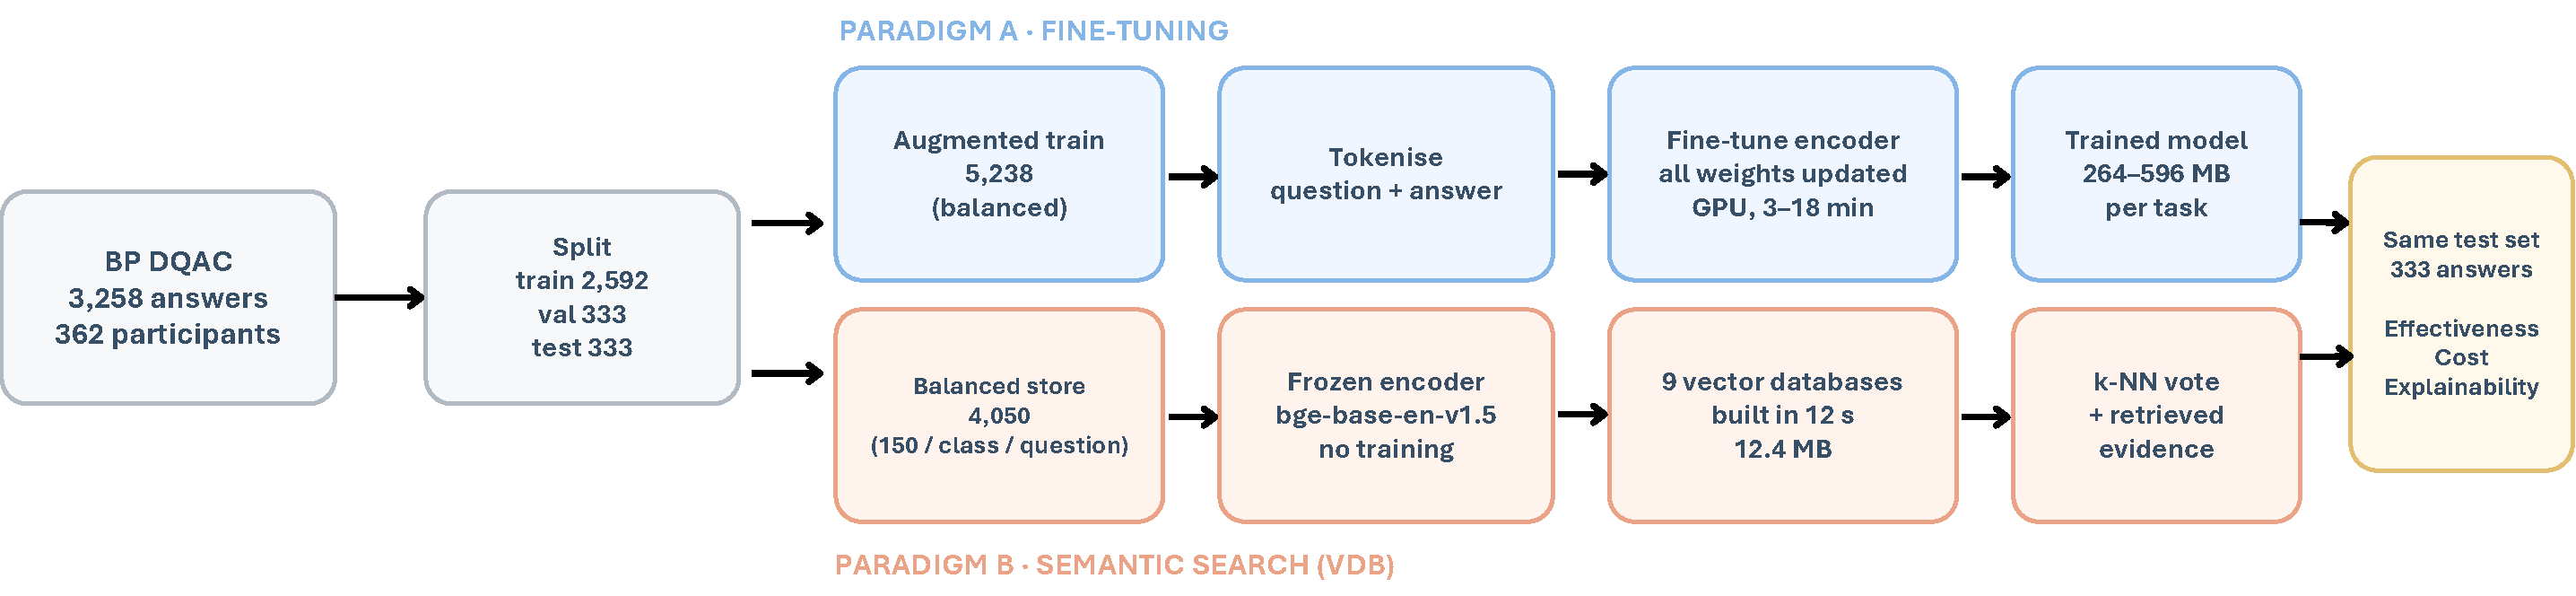
\includegraphics[width=\textwidth]{figures/study_design.pdf}
\caption{Study design. The two paradigms start from the same data and are evaluated on the same
held-out test set. Paradigm A learns new weights for the task. Paradigm B keeps the encoder frozen
and only stores labelled vectors.}
\label{fig:design}
\end{figure}

\subsection{Paradigm A: fine-tuned transformer encoders}

\paragraph{Why this baseline.}
Fine-tuned encoders are the standard way to build a text classifier. As Section~\ref{sec:lit}
shows, they usually match or beat prompted LLMs on classification. So they are the fairest and
strongest comparison for a training-free method.

\paragraph{Workflow.}
Figure~\ref{fig:baseline_workflow} shows the baseline workflow of our project. It has two parts. The
top row covers the data work. The bottom row covers model training and evaluation.

The data work starts with the questionnaire. We prepared it together with psychologists and
psychiatrists. We then collected answers from the participants. Experts checked every label. Then
semi-supervised learning spread these labels to the rest of the data (Section~\ref{sec:dataset}).
Next comes text cleaning. We make the text lower case and remove extra special characters. We expand
contractions. We replace common slang with the help of a hand-made dictionary. NLP preprocessing
then turns the text into model input. The question and the answer go in together as a pair. This
way the model knows which symptom the answer is about. The last step in the top row is class
imbalance. We used text augmentation and per-question balancing, on the training split only. (Weighted
loss was tried during development. The results here use the balanced set and no class weights.)

\begin{figure}[H]
\centering
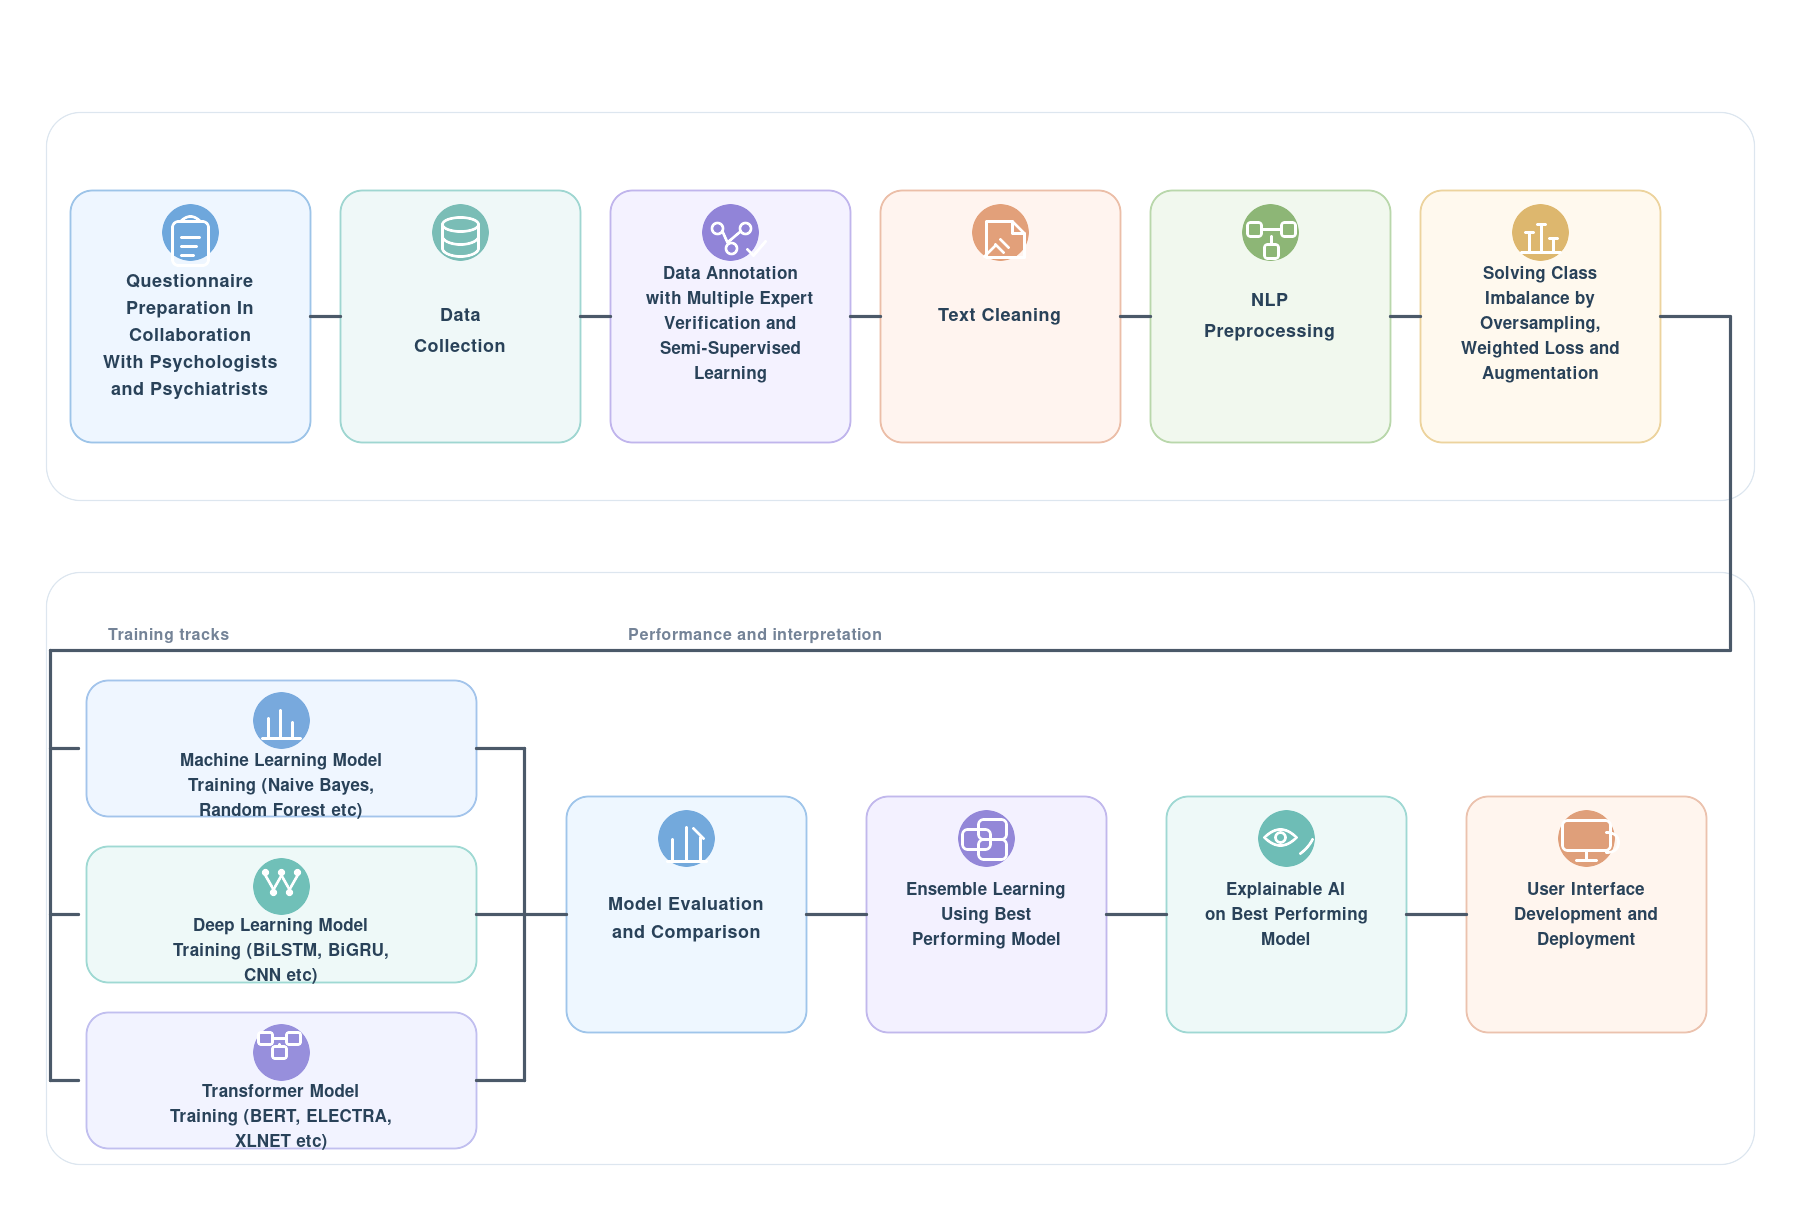
\includegraphics[width=0.98\textwidth]{figures/methodology_workflow_v4.png}
\caption{Baseline methodology workflow of the project. The upper row shows dataset construction and
preparation. The lower row shows model training, evaluation and deployment. This paper uses the
transformer track and the model evaluation step.}
\label{fig:baseline_workflow}
\end{figure}

The bottom row shows three training tracks: classical machine learning, deep learning and
transformers. This paper uses only the transformer track. The model evaluation step then scores all
models on the same test set. Ensemble learning, explainable AI and the user interface are later
stages of the wider project. They are outside the experiments reported here.

\paragraph{Models.}
We fine-tuned seven pretrained encoders. They cover different design ideas: BERT-base
(110M parameters)~\cite{devlin2019bert}, DistilBERT (67M, a distilled BERT)~\cite{sanh2019distilbert},
RoBERTa-base (125M), ELECTRA-base (110M), XLNet-base (117M), DeBERTa-v3-base (184M),
and ModernBERT-base (150M, a recent encoder with longer
context)~\cite{warner2024modernbert}. A linear layer with three outputs sits on top of the pooled
representation. The whole network is trained with cross-entropy loss.

\paragraph{Training decisions.}
We trained all models with the Hugging Face \texttt{Trainer} on the 4,050-answer balanced set. We
allowed at most 15 epochs. The effective batch size was 16 (we used gradient accumulation where
memory was short). The learning rate was $5\times10^{-6}$ for ELECTRA, BERT, DistilBERT, RoBERTa
and XLNet, and $2\times10^{-5}$ for DeBERTa-v3 and ModernBERT. Training stopped early if the
validation loss did not improve for two epochs, and we kept the checkpoint with the lowest
validation loss. Every model was trained three times (seeds 42, 43 and 44). We report mean
$\pm$ standard deviation. All runs used a single NVIDIA Tesla T4 GPU with fp16 mixed precision,
except DeBERTa-v3, which could not train in fp16 and used fp32.

\subsection{Paradigm B: Vector-Based Retrieval Inference (\vbri{})}

\paragraph{Why semantic search.}
The idea behind \vbri{} is simple. An embedding model already puts answers with similar meaning
close together. Experts have already labelled many answers. We store these. To classify a new
answer, we look up its closest stored answers and let them vote. Nothing is trained. The only
``learning'' is writing labelled vectors into a database. This gives four practical benefits for
clinical screening on limited hardware. (1) There is no GPU training. (2) One frozen encoder can
serve any number of tasks. (3) We update the system by adding or removing rows, not by retraining.
(4) Every prediction has a built-in explanation, since the retrieved answers can be shown to the
clinician. Figure~\ref{fig:vbri_arch} shows the full architecture.

% TODO(figure): vbri_architecture.pdf shows k = 5 and "5 retrieved"; the final run uses k = 3.
\begin{figure}[H]
\centering
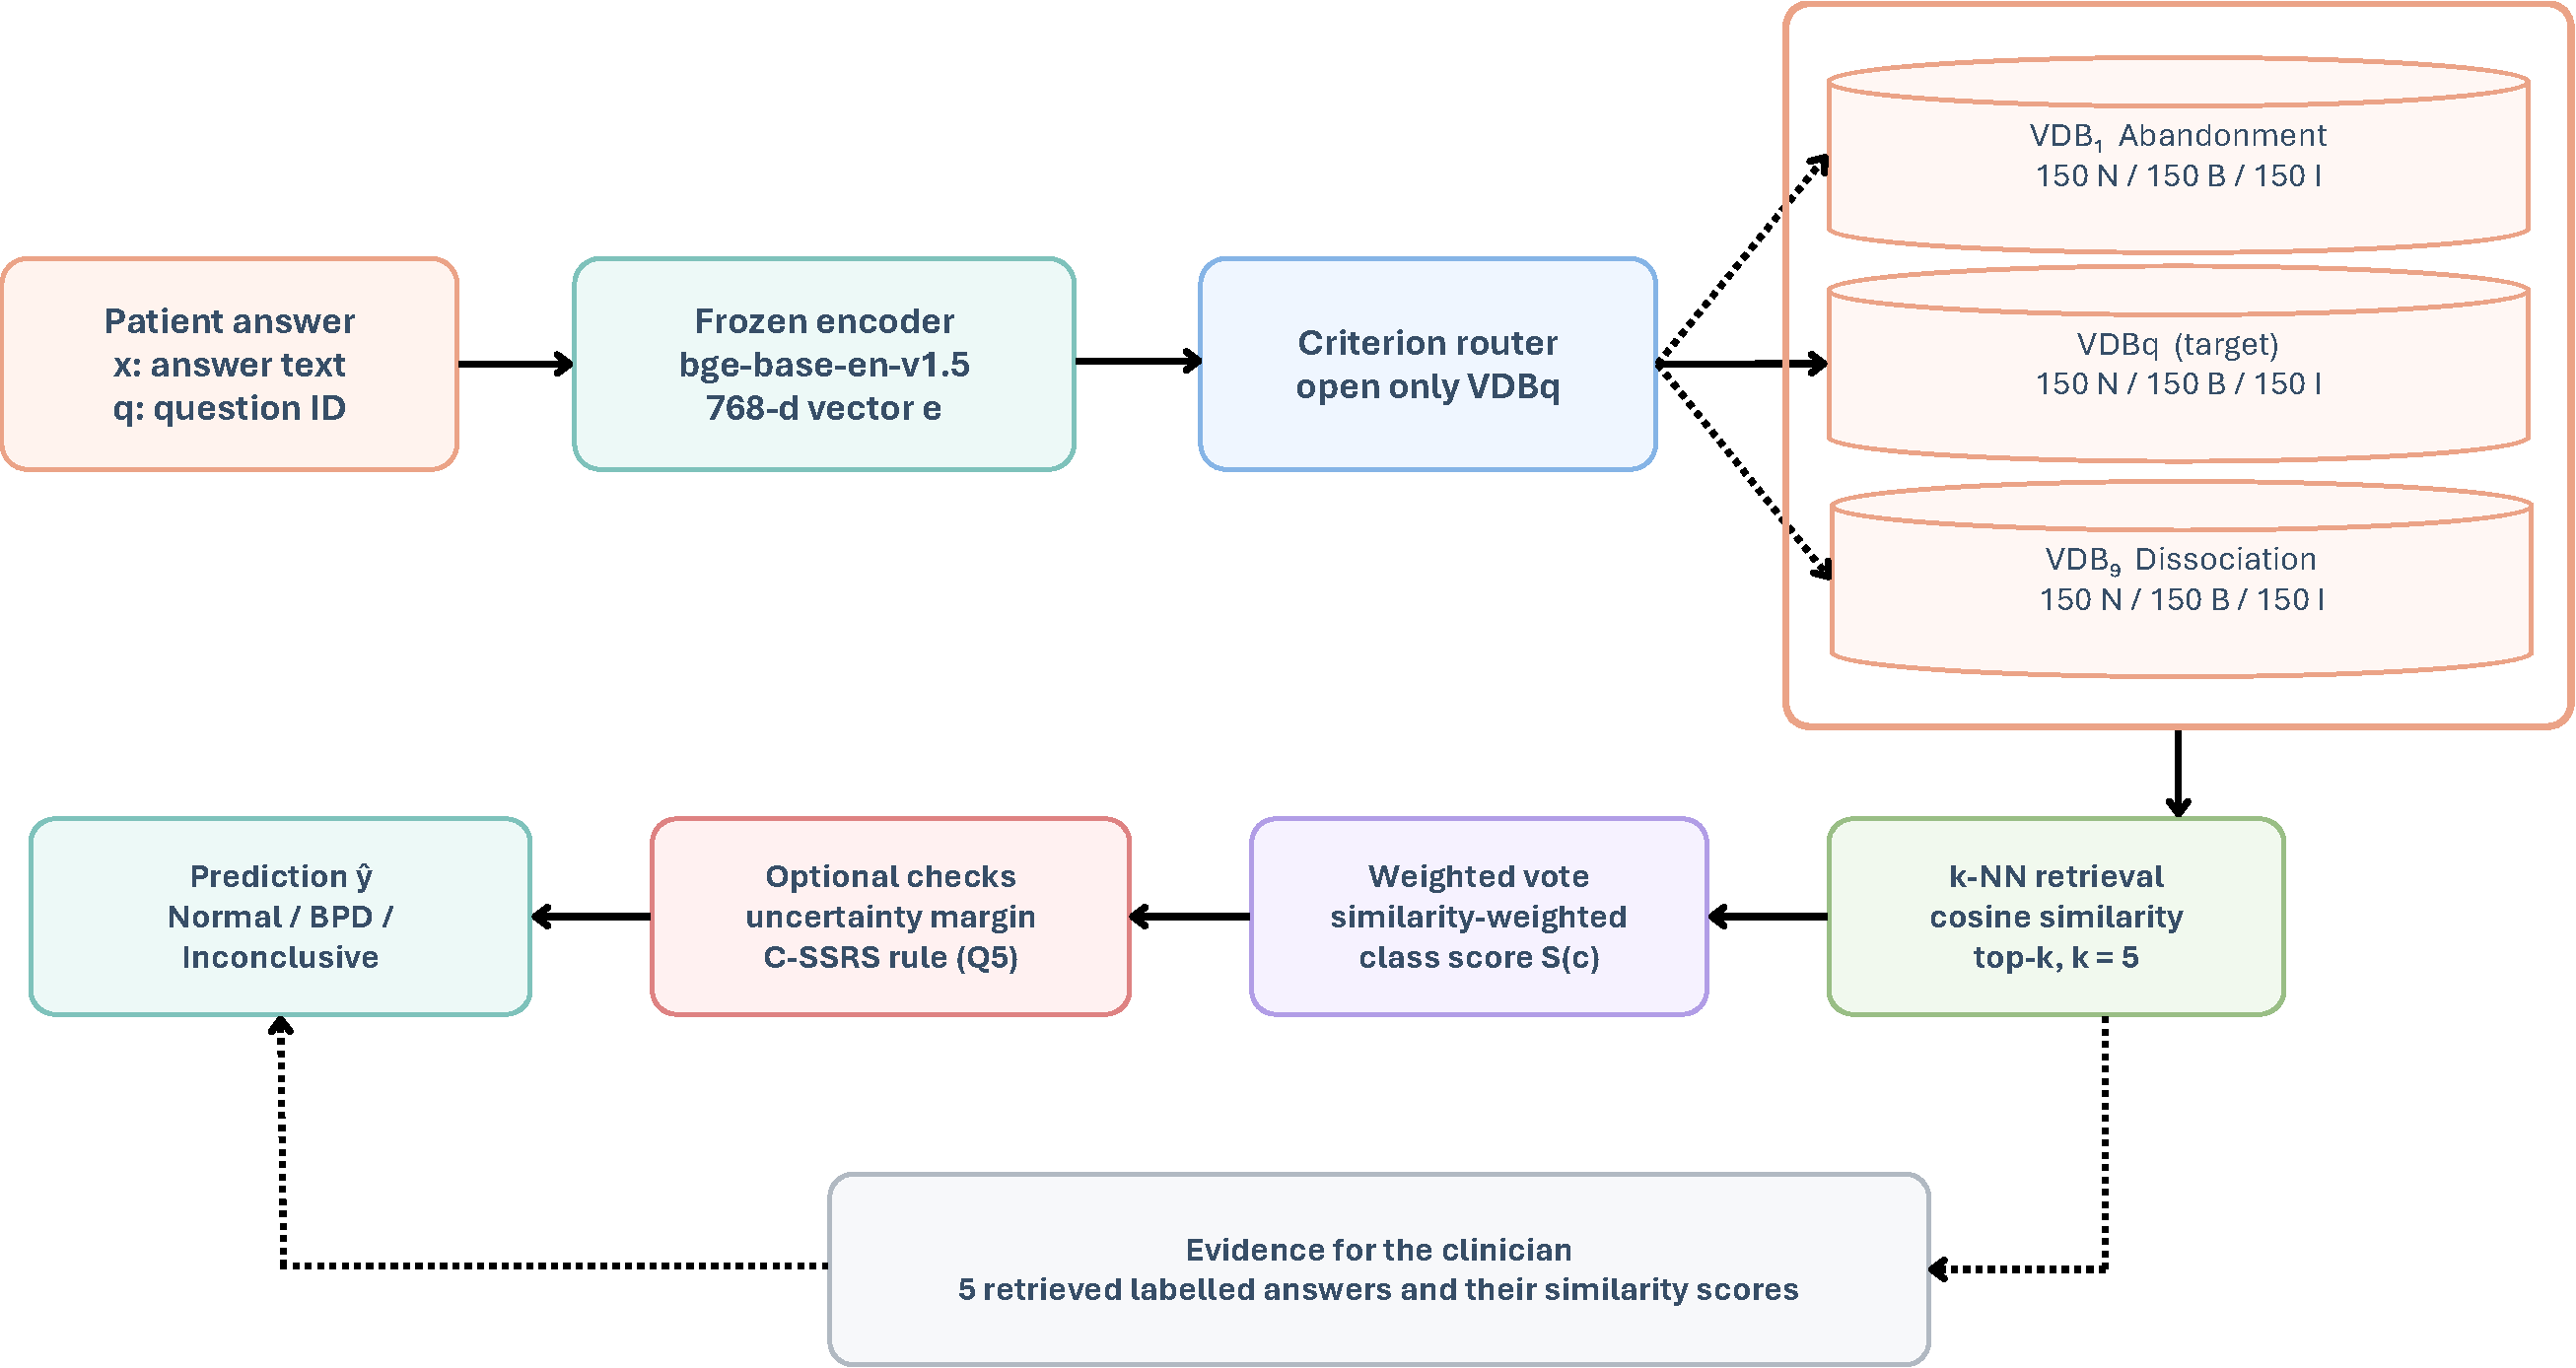
\includegraphics[width=0.92\textwidth]{figures/vbri_architecture.pdf}
\caption{\textbf{\vbri{} architecture.} An answer is encoded by a frozen embedding model and sent
only to the vector database of its own criterion. The top-$k$ most similar stored answers vote,
weighted by similarity. The retrieved answers double as an explanation of the decision.}
\label{fig:vbri_arch}
\end{figure}

\paragraph{Step 1: encoding with a frozen model.}
Every stored answer and every new answer is encoded once with \texttt{BAAI/bge-base-en-v1.5}
(109M parameters)~\cite{xiao2023cpack}. It gives 768-dimensional, unit-length vectors. We tested
four frozen encoders (MiniLM, MPNet, PubMedBERT and BGE), each with the answer alone or with the
question and the answer (Section~\ref{sec:encoder_text}). BGE with the answer alone gave the best
pooled test results and was tied with MPNet on validation. We use it in \vbri{}.

\paragraph{Step 2: one vector database per criterion (decision: isolation).}
Our first version kept all answers in one pooled index. It had a problem. Answers to different questions
share the same emotional words, such as ``empty'', ``hurt'', ``alone'' and ``angry''. So an answer
about anger often pulled neighbours from the emptiness or mood-instability questions. We now build
nine separate databases, $VDB_1$ to $VDB_9$. Each new answer goes only to the database of its own
question. In a structured interview the question is always known. So this routing is exact and
costs nothing.

\paragraph{Step 3: equal classes in every database (decision: balance).}
A $k$NN vote leans toward whichever class has more stored examples nearby. Inside one criterion, the
natural imbalance can be large. For example, the suicidal behaviour criterion had 259 Normal but
only 54 BPD answers in the unbalanced augmented set. So we fill each database with exactly 150
Normal, 150 BPD and 150 Inconclusive answers. This gives 450 per database and 4,050 in total
(Section~\ref{sec:dataset}).

\paragraph{Step 4: similarity-weighted $k$NN vote.}
Take a new answer with embedding $\mathbf{e}$ to question $q$. We compute the cosine similarity
$s_j = \mathbf{e}^\top \mathbf{e}_j$ to every vector in $VDB_q$. We keep the $k$ most similar and
score each class $c$ as
\begin{equation}
S(c) = \sum_{j \in \mathcal{N}_k} \max(s_j, 0)\cdot \mathbb{1}[y_j = c].
\label{eq:voting}
\end{equation}
The class with the highest score is the prediction. Weighting by similarity gives close neighbours
more say than distant ones. We chose $k$ from $\{1,3,5,7,9,11,15\}$ by macro F1 on the validation set, which gave $k=3$
(Figure~\ref{fig:ksweep}).

\paragraph{Step 5 (optional): uncertainty margin.}
Sometimes the two best classes get almost the same score. Then the evidence is truly mixed. The
calibrated variant turns the similarities of the $k$ neighbours into class proportions with a
temperature-scaled softmax,
\begin{equation}
P(c) = \frac{\sum_{j \in \mathcal{N}_k} \exp\big((s_j - s_{\max})/\tau\big)\,\mathbb{1}[y_j=c]}
            {\sum_{j \in \mathcal{N}_k} \exp\big((s_j - s_{\max})/\tau\big)}.
\end{equation}
It returns Inconclusive when the gap between the two largest values is below $\delta$. Otherwise it
returns BPD if $P(\text{BPD})\ge\theta$, and the larger of Normal and Inconclusive if not. A grid
search on the validation set gave $\tau=0.15$, $\delta=0.12$ and $\theta=0.40$.

\paragraph{Step 6 (optional): suicide-attempt safety rule.}
Embeddings can miss short but critical statements, and negation (Section~\ref{sec:lit}). For the
suicidal and self-harm criterion only, the hybrid variant uses a small set of regular expressions.
They are based on the ``actual attempt'' categories of the Columbia--Suicide Severity Rating Scale
(C-SSRS)~\cite{posner2011cssrs}, for example ``tried to hang myself'' or ``swallowed pills''. If a
pattern matches and the vote says Normal, we change the prediction to BPD. The rule can only move a
prediction toward the safer, positive class.

\paragraph{What is and is not tuned.}
\vbri{} has no trainable parameters. It has a few settings: $k$, and for the calibrated variant
$\tau$, $\delta$ and $\theta$. All of them were chosen on the validation set only. Two things came
from earlier development, where test results had already been seen: the choice of the BGE encoder,
and the C-SSRS rule, which was written after we looked at one missed test case. We therefore treat
the \emph{raw} configuration (isolation, balance, $k=3$, no margin, no rule) as the main
training-free result. The calibrated and hybrid variants are exploratory.

\subsection{Baselines inside Paradigm B}

To show which parts of \vbri{} matter, we also test simpler retrieval classifiers. They use one
pooled index of the balanced set for all questions. We tried dense retrieval with MiniLM, MPNet,
PubMedBERT and BGE (with answer-only or question+answer text), and two lexical methods, BM25 and
TF-IDF. For every baseline, $k$ was chosen on the validation set in the same way as for \vbri{}.

\subsection{Evaluation protocol}

\paragraph{Effectiveness.} We report accuracy, macro F1 (which weights the three classes equally),
weighted F1, BPD F1 and BPD sensitivity (the recall of the BPD class). For screening, BPD
sensitivity is the most important number. A missed BPD answer is a person who may not be referred
for assessment. We also report a binary BPD-versus-rest view. It has specificity, positive and
negative predictive values (PPV, NPV) and the diagnostic odds ratio (DOR).

\paragraph{Cost.} We report three things, all measured on the same machine. (i) \emph{Training or
index-build time}: the wall-clock time of the \texttt{Trainer} run (including per-epoch evaluation
and checkpoint saving), or the time to encode all 4,050 stored answers (median of three runs; model
loading not counted). (ii) \emph{Inference time per answer}, from text to prediction: on the GPU with
batch size 1 and 32, and on the CPU with batch size 1. (iii) \emph{Task-specific storage}: the fp32
model weights for fine-tuning and the vector index for \vbri{}. The \vbri{} encoder is frozen and can
be shared by several tasks, so it is not counted as task-specific. It still has to be present on the
device (about 438\,MB in fp32).

\paragraph{Contamination.} For pooled retrieval, we measure the share of the top-$k$ neighbours that
come from a different question than the query. For \vbri{}, this is 0\% by design.

\paragraph{Statistics.} We compare paired predictions with the exact McNemar
test~\cite{mcnemar1947} and give 95\% confidence intervals from 10,000 paired bootstrap samples of
the test set. For these paired comparisons we use one fine-tuned model, chosen by mean validation
macro F1 (ELECTRA, seed 42). Accuracy should be read with care: always answering Normal already
gives 67.57\% on this test set.

% =============================================================================
% 5. RESULTS
% =============================================================================
\section{Results}\label{sec:results}

\subsection{How the fine-tuned models learned}

Figure~\ref{fig:loss} shows the training and validation loss of each fine-tuned model (seed 42). The
training loss keeps falling. The validation loss reaches its lowest value after 3 to 7 epochs and
then rises or stays flat. This is the usual sign of overfitting on a small dataset. Early stopping
kept the best checkpoint (dotted line). Over the three seeds, the models needed 4.7 to 8.0 epochs on
average.

\begin{figure}[H]
\centering
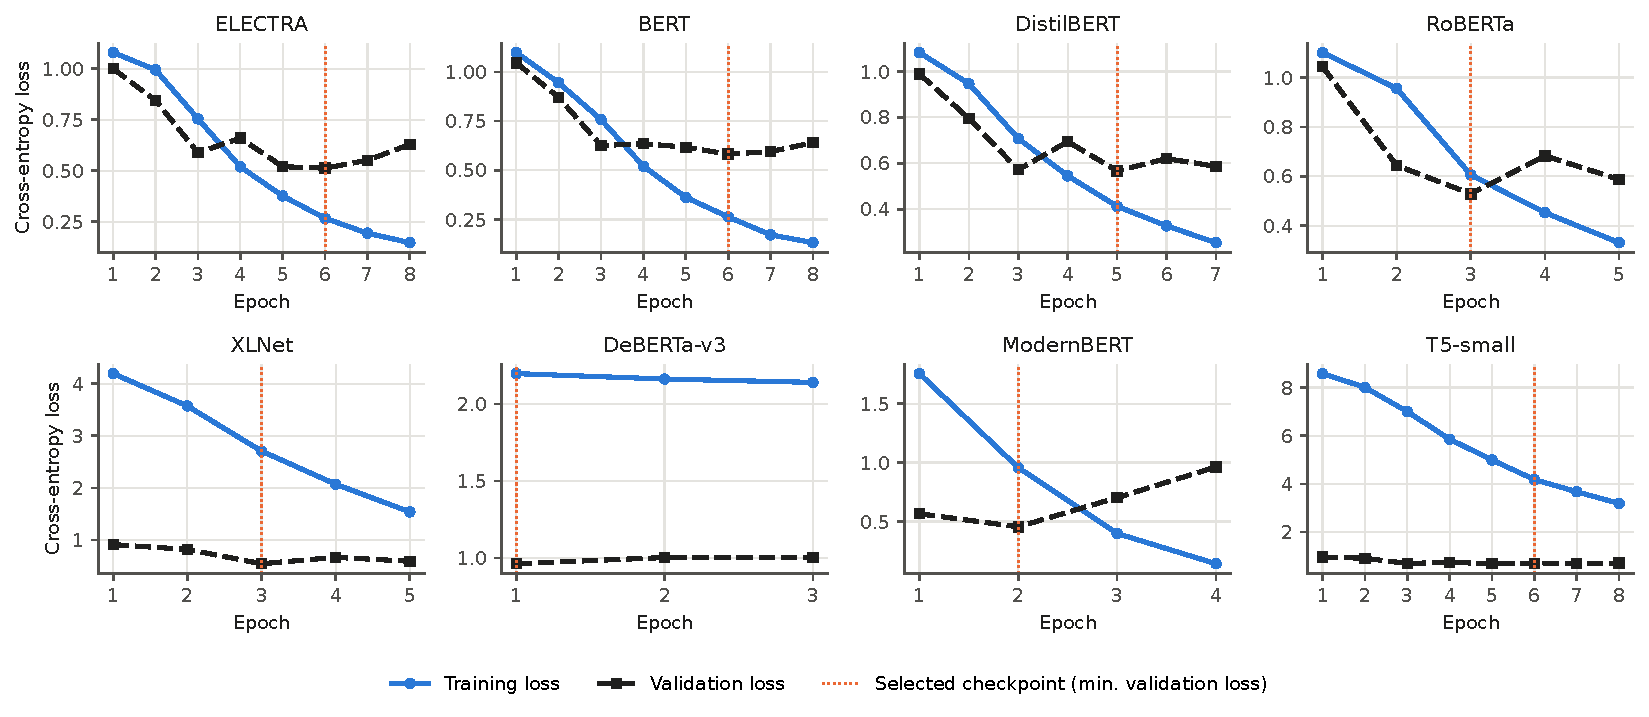
\includegraphics[width=\textwidth]{figures/generated/ft_loss_curves.pdf}
\caption{Training and validation loss per epoch for the seven fine-tuned models (seed 42, Tesla T4).
The dotted line marks the checkpoint with the lowest validation loss.}
\label{fig:loss}
\end{figure}

Table~\ref{tab:encoder_results} and Figure~\ref{fig:ft_cm} give the test results. ModernBERT has the
highest mean accuracy (84.78\%). ELECTRA is very close (83.88\%), is more stable across seeds and has
the highest mean macro F1 (78.25\%) and BPD sensitivity (85.07\%). ELECTRA also had the highest mean
validation macro F1, so we use it as the best fine-tuned model. The spread between seeds is large for
some models, especially in BPD sensitivity (up to $\pm$9.8 points). A single run can therefore be
misleading. A bigger model is not always better: DeBERTa-v3 is the largest and the weakest.

\begin{table}[H]
\centering
\caption{Fine-tuned encoders on the \bpdqac{} test set ($N=333$), mean $\pm$ standard deviation
over three seeds. Values in \%, except training time (seconds on one Tesla T4) and epochs.}
\label{tab:encoder_results}
\scriptsize
\setlength{\tabcolsep}{3pt}
\renewcommand{\arraystretch}{1.2}
\resizebox{\textwidth}{!}{%
\begin{tabular}{@{}lccccccccc@{}}
\toprule
\textbf{Model} & \textbf{Params} & \textbf{Prec.} & \textbf{Train time (s)} & \textbf{Epochs} & \textbf{Accuracy} & \textbf{Weighted F1} & \textbf{Macro F1} & \textbf{BPD F1} & \textbf{BPD Sens.} \\
\midrule
ELECTRA & 110M & fp16 & 275 $\pm$ 20 & 7.7 $\pm$ 0.6 & 83.88 $\pm$ 1.21 & 84.17 $\pm$ 1.08 & 78.25 $\pm$ 1.58 & 75.13 $\pm$ 1.02 & 85.07 $\pm$ 7.76 \\
BERT & 110M & fp16 & 284 $\pm$ 35 & 8.0 $\pm$ 1.0 & 78.48 $\pm$ 0.63 & 79.26 $\pm$ 0.52 & 73.14 $\pm$ 1.23 & 67.96 $\pm$ 1.98 & 79.10 $\pm$ 1.49 \\
DistilBERT & 67M & fp16 & 116 $\pm$ 9 & 6.3 $\pm$ 0.6 & 74.07 $\pm$ 2.77 & 75.42 $\pm$ 2.48 & 67.82 $\pm$ 1.98 & 64.39 $\pm$ 1.72 & 78.61 $\pm$ 9.00 \\
RoBERTa & 125M & fp16 & 211 $\pm$ 14 & 5.7 $\pm$ 0.6 & 76.48 $\pm$ 2.79 & 77.88 $\pm$ 2.41 & 70.78 $\pm$ 2.19 & 70.81 $\pm$ 1.69 & 82.59 $\pm$ 1.72 \\
XLNet & 117M & fp16 & 509 $\pm$ 72 & 7.0 $\pm$ 1.0 & 80.68 $\pm$ 2.13 & 81.00 $\pm$ 1.96 & 73.41 $\pm$ 2.85 & 72.19 $\pm$ 2.32 & 78.61 $\pm$ 4.56 \\
DeBERTa & 184M & fp32 & 796 $\pm$ 130 & 6.0 $\pm$ 1.0 & 70.87 $\pm$ 4.48 & 71.87 $\pm$ 3.89 & 63.72 $\pm$ 1.86 & 57.36 $\pm$ 2.96 & 77.61 $\pm$ 9.79 \\
ModernBERT & 150M & fp16 & 277 $\pm$ 39 & 4.7 $\pm$ 0.6 & 84.78 $\pm$ 2.72 & 84.50 $\pm$ 3.07 & 77.73 $\pm$ 5.96 & 75.10 $\pm$ 2.10 & 77.61 $\pm$ 9.32 \\
\bottomrule
\end{tabular}
}
\end{table}

\begin{figure}[H]
\centering
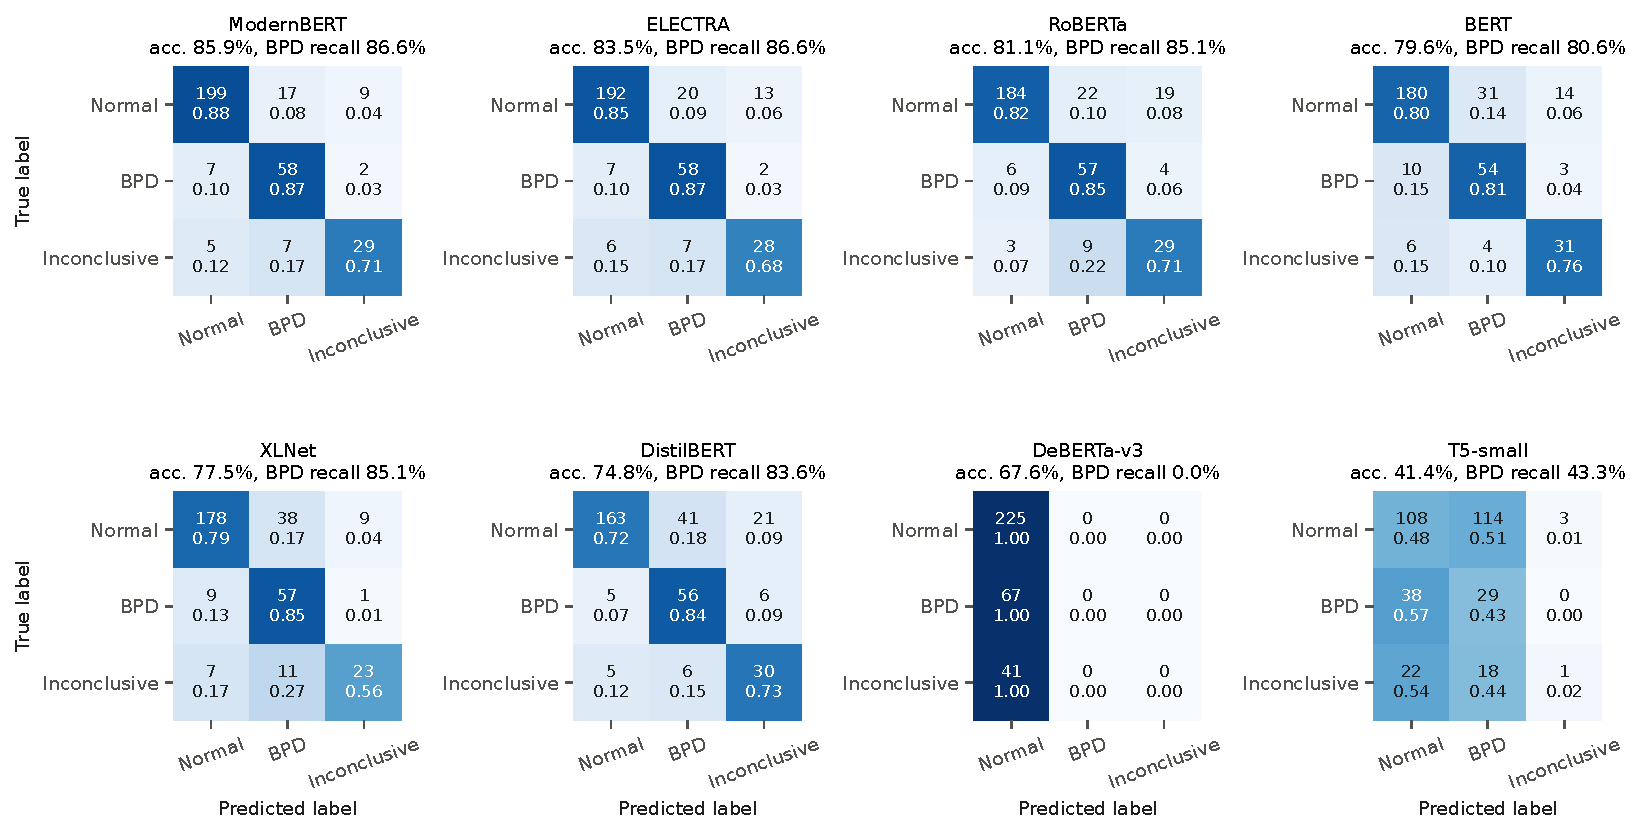
\includegraphics[width=\textwidth]{figures/generated/ft_confusion_matrices.pdf}
\caption{Test confusion matrices of the seven fine-tuned models for seed 42 (counts and
row-normalised proportions).}
\label{fig:ft_cm}
\end{figure}

\subsection{Choosing the encoder and the input text}\label{sec:encoder_text}

We compared four frozen encoders, each with two input texts: the answer alone, and the question plus
the answer. All eight runs used one pooled index of the 4,050 balanced answers and the same test
set, with $k$ chosen on validation. Figure~\ref{fig:encoder_text} shows the results. With the answer
alone, BGE was the best encoder (67.27\% accuracy, 57.26\% macro F1). MiniLM followed in accuracy
(64.26\%), then MPNet (63.36\%) and PubMedBERT (61.86\%). On the validation set, MPNet and BGE were
tied (macro F1 64.07\% and 63.92\%).

\begin{figure}[H]
\centering
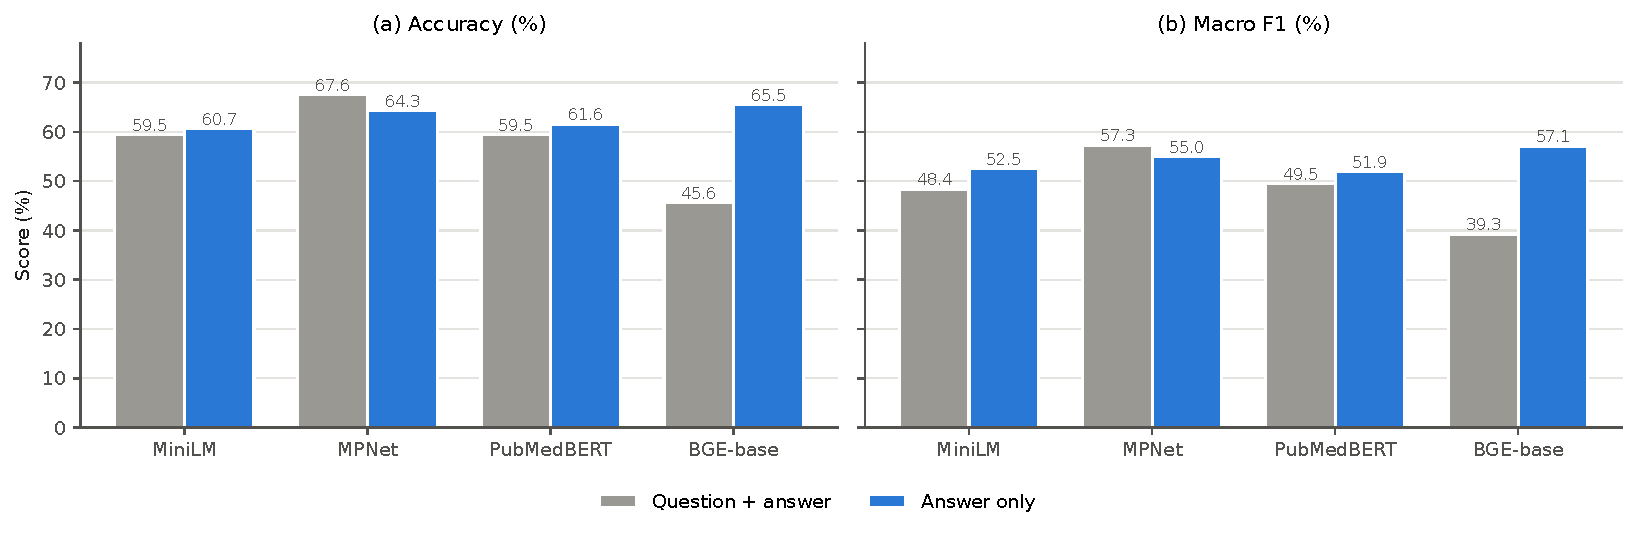
\includegraphics[width=\textwidth]{figures/generated/encoder_input_text.pdf}
\caption{Effect of the input text on four frozen encoders (pooled balanced index, $k$ chosen on
validation, $N=333$). (a) Accuracy. (b) Macro F1.}
\label{fig:encoder_text}
\end{figure}

Adding the question text lowered accuracy for three of the four encoders: BGE from 67.27\% to
60.36\%, MiniLM from 64.26\% to 60.96\%, and PubMedBERT from 61.86\% to 61.26\%. MPNet moved the
other way, from 63.36\% to 66.67\%. So the effect depends on the encoder. With the question included,
all neighbours came from the same question (0\% contamination), yet the results did not improve in
general. A likely reason is that the shared question text pulls the vectors of one question together
and hides the differences between answers. We did not test this explanation directly. \vbri{} encodes
the answer alone.

\subsection{Cross-criterion contamination in a pooled index}

The simplest semantic search classifier uses one pooled BGE index over all questions. It reaches
67.27\% accuracy and 57.26\% macro F1 (Table~\ref{tab:master}), no better in accuracy than always
answering Normal (67.57\%), although it does find 65.67\% of the BPD answers. One reason is visible in
Figure~\ref{fig:contam}b. At $k=3$, 35.6\% of the retrieved neighbours come from a \emph{different}
question than the query. For abandonment (Q1) it is 43.2\%. These neighbours carry labels that were
given for a different symptom. All pooled answer-only and lexical baselines show contamination, from
28.2\% to 56.6\%.

\begin{figure}[H]
\centering
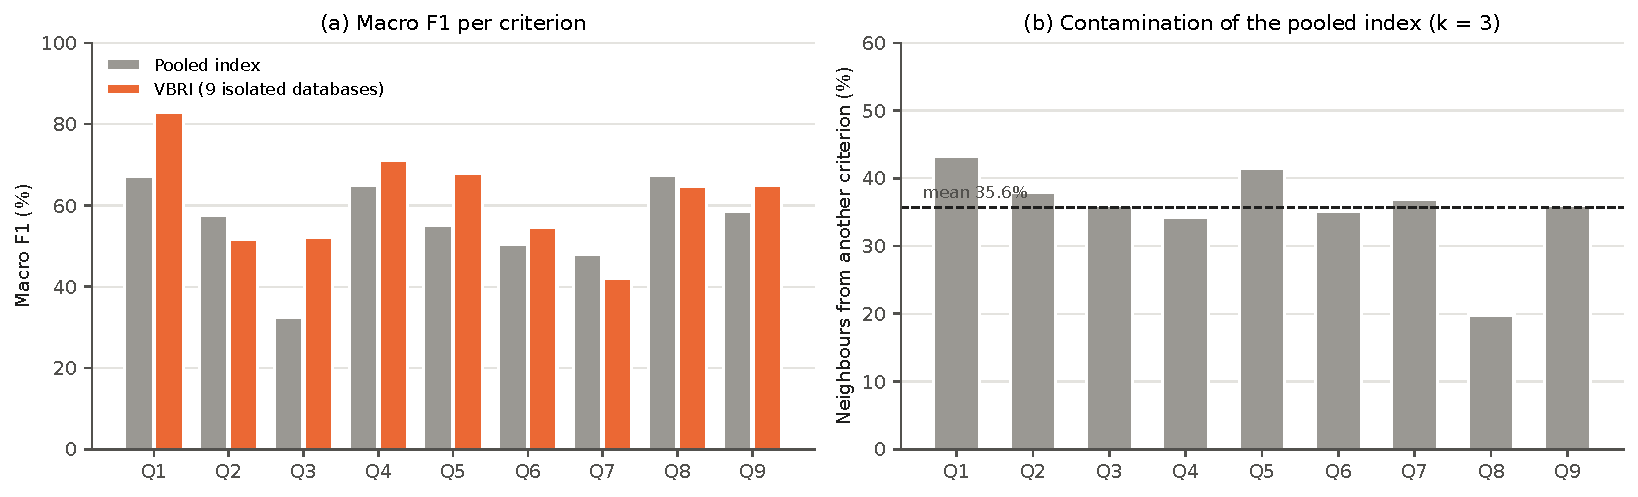
\includegraphics[width=\textwidth]{figures/generated/contamination_per_criterion.pdf}
\caption{(a) Macro F1 per criterion for the pooled index and \vbri{} ($k=3$). (b) Share of retrieved
neighbours that come from the wrong criterion in the pooled index. For \vbri{} it is 0\% by design.}
\label{fig:contam}
\end{figure}

\subsection{What isolation and balance change}

Table~\ref{tab:ablation} and Figure~\ref{fig:ablation} separate the two design decisions, all with
$k=3$. The clearest effect is on BPD sensitivity. Isolating the criteria raised it in all three
settings: from 76.12\% to 79.10\% with the unbalanced set, from 73.13\% to 80.60\% with class
weights, and from 71.64\% to 80.60\% with the balanced set. The effect on accuracy is small. All six
configurations lie between 67.27\% and 70.57\%. \vbri{} raw is 3.3 points above the balanced pooled
index, which is not statistically significant (exact McNemar $p=0.09$). Class weights on the
unbalanced set give almost the same result as balancing (69.97\% accuracy, 80.60\% sensitivity).

\begin{table}[H]
\centering
\caption{Ablation of \vbri{} design decisions (BGE-base, answer only, $k=3$, $N=333$). Values in \%.}
\label{tab:ablation}
\small
\setlength{\tabcolsep}{4pt}
\resizebox{\textwidth}{!}{%
\begin{tabular}{@{}lcccccc@{}}
\toprule
\textbf{Configuration} & \textbf{Vectors} & \textbf{Isolation} & \textbf{Balance} & \textbf{Accuracy} & \textbf{Macro F1} & \textbf{BPD Sens.} \\
\midrule
Pooled, unbalanced & 4,279 & -- & -- & 69.07 & 60.45 & 76.12 \\
Isolated, unbalanced & 4,279 & \checkmark & -- & 69.07 & 58.28 & 79.10 \\
Pooled, unbalanced + class weights & 4,279 & -- & weights & 69.07 & 60.95 & 73.13 \\
Isolated, unbalanced + class weights & 4,279 & \checkmark & weights & 69.97 & 61.44 & 80.60 \\
Pooled, balanced & 4,050 & -- & \checkmark & 67.27 & 59.08 & 71.64 \\
Isolated, balanced (VBRI raw) & 4,050 & \checkmark & \checkmark & 70.57 & 63.16 & 80.60 \\
\quad + uncertainty margin ($\tau$=0.15, $\delta$=0.12, $\theta$=0.4) & 4,050 & \checkmark & \checkmark & 70.87 & 64.24 & 80.60 \\
\quad + C-SSRS rule (hybrid) & 4,050 & \checkmark & \checkmark & 71.17 & 64.57 & 82.09 \\
\bottomrule
\end{tabular}
}
\end{table}

\begin{figure}[H]
\centering
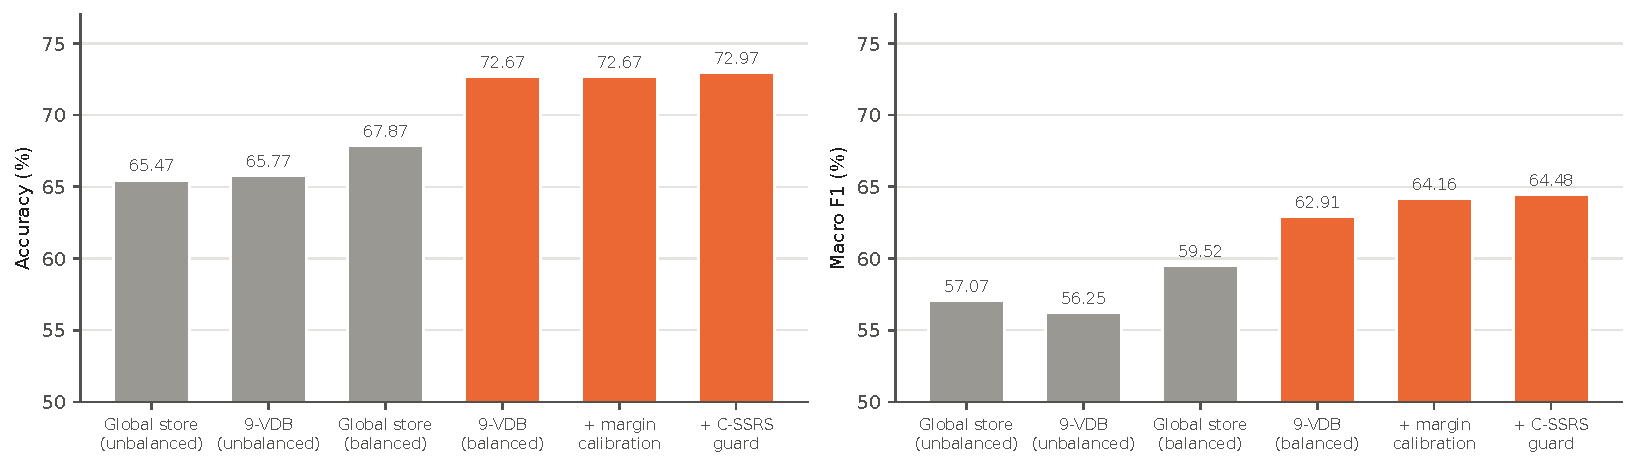
\includegraphics[width=\textwidth]{figures/generated/ablation_progression.pdf}
\caption{Accuracy, macro F1 and BPD sensitivity across the ablation. Grey bars lack isolation or
per-question balance. Orange bars have both.}
\label{fig:ablation}
\end{figure}

The two optional steps add little. The calibrated variant changes three test predictions (two fixed,
one broken; exact McNemar $p=1.00$). Inconclusive recall rises from 48.8\% to 53.7\% and macro F1 by
1.08 points. The C-SSRS rule fired on one test answer and on no validation answer. It was a true
suicide-attempt disclosure (``I did try to hang myself from the ceiling fan'') that the vote had
called Normal. One correct override cannot prove that the rule works.

Figure~\ref{fig:ksweep} shows the effect of $k$. On the test set, \vbri{} has a higher macro F1 than
the pooled index for $k$ from 1 to 7, but not for all larger values. On the validation set the order
is reversed: the pooled index has the higher macro F1 at every $k$. At the chosen settings,
validation macro F1 is 63.92\% for the pooled index and 60.44\% for \vbri{}, while validation BPD
sensitivity is 70.59\% and 86.76\%. So the gain in BPD sensitivity appears in both sets. A gain in
overall quality does not.

\begin{figure}[H]
\centering
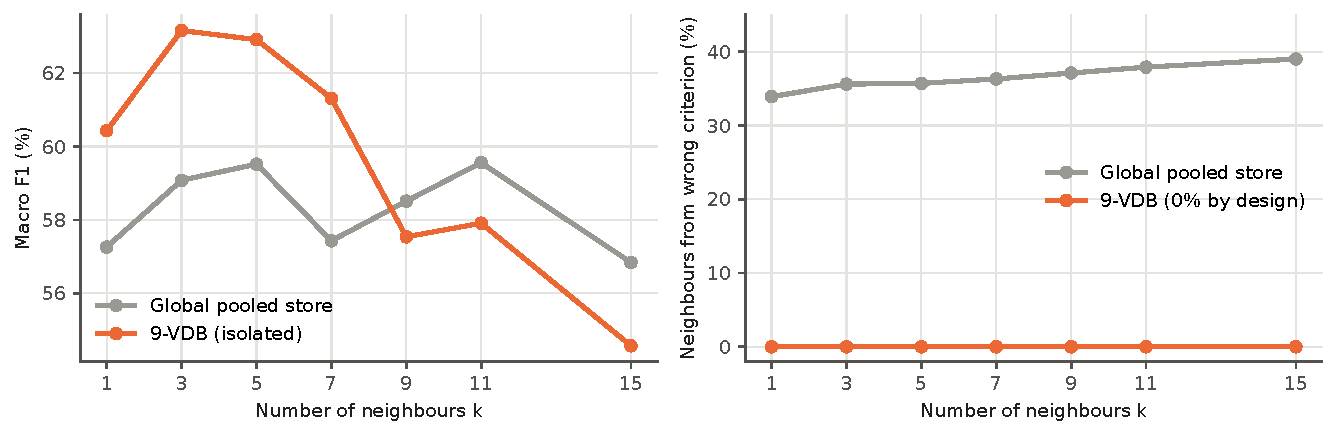
\includegraphics[width=\textwidth]{figures/generated/k_sweep.pdf}
\caption{Effect of the number of neighbours $k$. Left: macro F1 on validation and test. Right:
share of neighbours retrieved from the wrong criterion.}
\label{fig:ksweep}
\end{figure}

\subsection{Head-to-head: fine-tuning versus semantic search}

Table~\ref{tab:master} and Figure~\ref{fig:effect} place all configurations side by side.

\begin{table}[H]
\centering
\caption{All configurations on the same test set ($N=333$). Fine-tuned rows are means over three
seeds. ``Contam.'' is the share of retrieved neighbours from the wrong criterion. Always answering
Normal gives 67.57\% accuracy, 26.88\% macro F1 and 0\% BPD sensitivity. Values in \%.}
\label{tab:master}
\scriptsize
\setlength{\tabcolsep}{3pt}
\renewcommand{\arraystretch}{1.1}
\resizebox{\textwidth}{!}{%
\begin{tabular}{@{}llccccccc@{}}
\toprule
\textbf{Paradigm} & \textbf{Model} & \textbf{Trainable} & \textbf{k} & \textbf{Contam.} & \textbf{Accuracy} & \textbf{Macro F1} & \textbf{BPD Sens.} & \textbf{BPD F1} \\
\midrule
Fine-tuned & ELECTRA & 110M & -- & N/A & 83.88 $\pm$ 1.21 & 78.25 $\pm$ 1.58 & 85.07 $\pm$ 7.76 & 75.13 $\pm$ 1.02 \\
Fine-tuned & BERT & 110M & -- & N/A & 78.48 $\pm$ 0.63 & 73.14 $\pm$ 1.23 & 79.10 $\pm$ 1.49 & 67.96 $\pm$ 1.98 \\
Fine-tuned & DistilBERT & 67M & -- & N/A & 74.07 $\pm$ 2.77 & 67.82 $\pm$ 1.98 & 78.61 $\pm$ 9.00 & 64.39 $\pm$ 1.72 \\
Fine-tuned & RoBERTa & 125M & -- & N/A & 76.48 $\pm$ 2.79 & 70.78 $\pm$ 2.19 & 82.59 $\pm$ 1.72 & 70.81 $\pm$ 1.69 \\
Fine-tuned & XLNet & 117M & -- & N/A & 80.68 $\pm$ 2.13 & 73.41 $\pm$ 2.85 & 78.61 $\pm$ 4.56 & 72.19 $\pm$ 2.32 \\
Fine-tuned & DeBERTa & 184M & -- & N/A & 70.87 $\pm$ 4.48 & 63.72 $\pm$ 1.86 & 77.61 $\pm$ 9.79 & 57.36 $\pm$ 2.96 \\
Fine-tuned & ModernBERT & 150M & -- & N/A & 84.78 $\pm$ 2.72 & 77.73 $\pm$ 5.96 & 77.61 $\pm$ 9.32 & 75.10 $\pm$ 2.10 \\
\midrule
Pooled dense & Pooled MiniLM (answer) & 0 & 1 & 32.7 & 64.26 & 53.30 & 46.27 & 40.00 \\
Pooled dense & Pooled MiniLM (Q+A) & 0 & 1 & 0.0 & 60.96 & 46.91 & 32.84 & 35.77 \\
Pooled dense & Pooled MPNet (answer) & 0 & 1 & 28.2 & 63.36 & 50.11 & 58.21 & 45.35 \\
Pooled dense & Pooled MPNet (Q+A) & 0 & 1 & 0.0 & 66.67 & 54.99 & 56.72 & 48.10 \\
Pooled dense & Pooled PubMedBERT (answer) & 0 & 1 & 38.4 & 61.86 & 49.96 & 61.19 & 50.62 \\
Pooled dense & Pooled PubMedBERT (Q+A) & 0 & 1 & 0.0 & 61.26 & 50.15 & 46.27 & 43.06 \\
Pooled dense & Pooled BGE (answer) & 0 & 1 & 33.9 & 67.27 & 57.26 & 65.67 & 56.41 \\
Pooled dense & Pooled BGE (Q+A) & 0 & 7 & 0.0 & 60.36 & 51.97 & 58.21 & 47.85 \\
\midrule
Pooled lexical & Pooled BM25 & 0 & 9 & 47.1 & 61.86 & 48.19 & 52.24 & 44.03 \\
Pooled lexical & Pooled TF-IDF & 0 & 15 & 56.6 & 63.66 & 51.24 & 43.28 & 43.94 \\
\midrule
\textbf{VBRI (ours)} & VBRI raw & 0 & 3 & 0.0 & 70.57 & 63.16 & 80.60 & 59.34 \\
\textbf{VBRI (ours)} & VBRI calibrated & 0 & 3 & 0.0 & 70.87 & 64.24 & 80.60 & 59.67 \\
\textbf{VBRI (ours)} & VBRI raw + C-SSRS & 0 & 3 & 0.0 & 70.87 & 63.48 & 82.09 & 60.11 \\
\textbf{VBRI (ours)} & VBRI hybrid & 0 & 3 & 0.0 & 71.17 & 64.57 & 82.09 & 60.44 \\
\bottomrule
\end{tabular}
}
\end{table}

\begin{figure}[H]
\centering
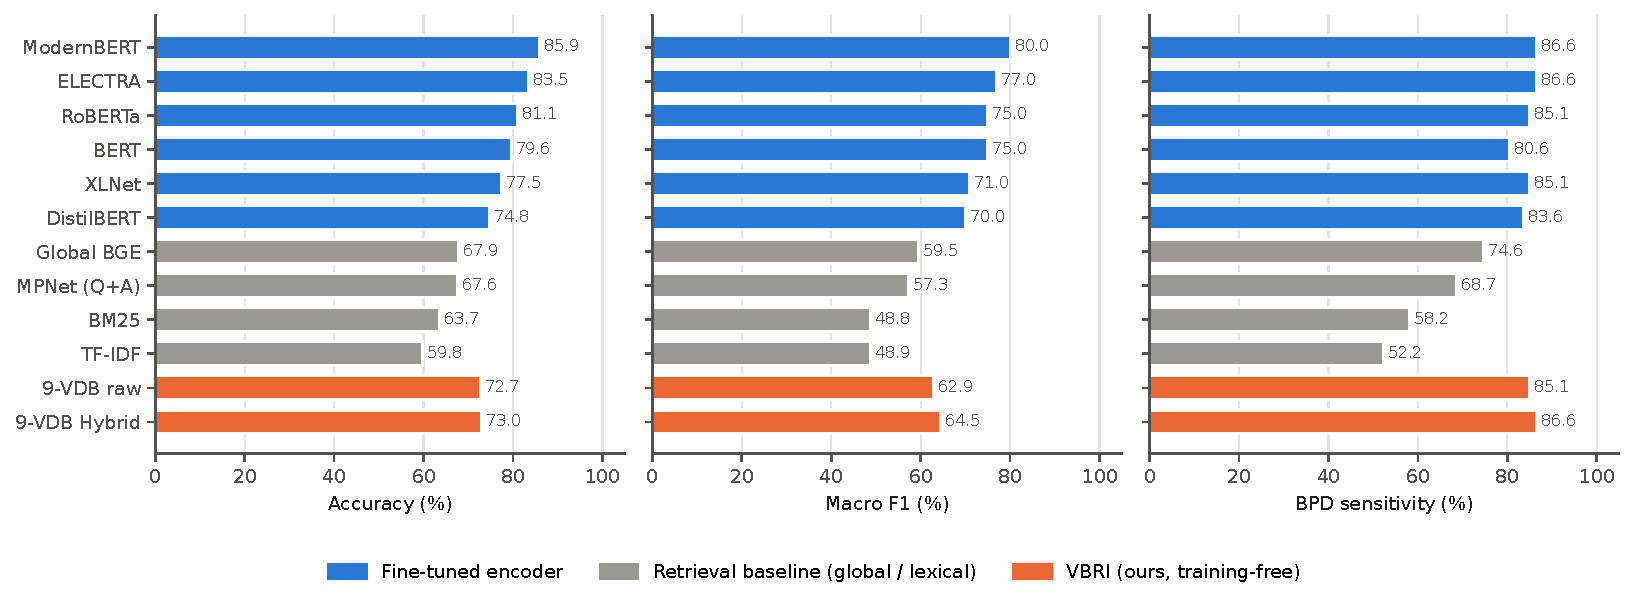
\includegraphics[width=\textwidth]{figures/generated/effectiveness_comparison.pdf}
\caption{Accuracy, macro F1 and BPD sensitivity of fine-tuned encoders (blue, mean $\pm$ sd over
three seeds), pooled retrieval baselines (grey) and \vbri{} (orange).}
\label{fig:effect}
\end{figure}

Three findings stand out.

\textbf{(1) On overall effectiveness, fine-tuning clearly wins.} ELECTRA is 13.3 points more
accurate than \vbri{} raw on average (83.88\% vs.\ 70.57\%) and its macro F1 is 15.1 points higher.
In the paired comparison (seed 42), the accuracy difference is 12.0 points (95\% CI 6.9 to 17.4;
exact McNemar $p<0.001$; Table~\ref{tab:bootstrap}).

\textbf{(2) On BPD sensitivity, semantic search is within the range of fine-tuning, but not at the
top (RQ1).} \vbri{} raw finds 54 of the 67 BPD answers (80.60\%). The seven fine-tuned means range
from 77.61\% to 85.07\%. \vbri{} is above five of them and below RoBERTa and ELECTRA. The ELECTRA run
used for the paired tests found 63 answers (94.03\%), significantly more than \vbri{} ($p=0.022$).
This is well above the ELECTRA three-seed mean (85.07\%), so the gap to a typical run is
smaller.

\textbf{(3) Isolation and balance help retrieval find BPD answers (RQ3).} The pooled baselines reach
32.84\% to 65.67\% BPD sensitivity. \vbri{} raw reaches 80.60\%. Against the pooled BGE baseline it
finds 12 BPD answers that the baseline missed and misses 2 that the baseline found (exact McNemar on
BPD answers, $p=0.013$). The price is more false alarms: specificity is 77.07\% against 83.08\%.

\begin{table}[H]
\centering
\caption{Paired bootstrap estimates with 95\% confidence intervals (10,000 samples). ELECTRA is the
seed-42 run. Values in \%.}
\label{tab:bootstrap}
\small
\resizebox{\textwidth}{!}{%
\begin{tabular}{@{}lcccc@{}}
\toprule
\textbf{Model / difference} & \textbf{Accuracy} & \textbf{Macro F1} & \textbf{BPD Sens.} & \textbf{Specificity} \\
\midrule
ELECTRA & 82.58 [78.38, 86.49] & 76.70 [70.85, 82.01] & 94.03 [87.69, 98.63] & 86.47 [82.20, 90.46] \\
VBRI raw & 70.57 [65.47, 75.38] & 63.16 [56.64, 69.10] & 80.60 [70.59, 89.71] & 77.07 [71.79, 81.92] \\
VBRI hybrid & 71.17 [66.37, 75.98] & 64.57 [58.07, 70.46] & 82.09 [72.22, 90.91] & 77.44 [72.14, 82.29] \\
Pooled BGE (answer) & 67.27 [62.16, 72.07] & 57.26 [50.64, 63.31] & 65.67 [54.29, 76.79] & 83.08 [78.46, 87.41] \\
\midrule
ELECTRA - VBRI raw & 12.01 [6.91, 17.42] & 13.54 [6.60, 20.69] & 13.43 [3.33, 23.88] & 9.40 [4.03, 15.04] \\
ELECTRA - VBRI hybrid & 11.41 [6.31, 16.82] & 12.13 [5.22, 19.18] & 11.94 [2.30, 22.22] & 9.02 [3.69, 14.70] \\
\bottomrule
\end{tabular}
}
\end{table}

Figure~\ref{fig:h2h} shows where the gap comes from. \vbri{} raw labels 49 Normal answers as BPD
(ELECTRA: 27) and finds fewer Inconclusive answers (20 vs.\ 26 of 41). Semantic search is good at
finding answers that \emph{sound like} BPD answers. A trained decision boundary is better at
separating ordinary distress from true pathology. The ROC curves in Figure~\ref{fig:roc} agree: the
area under the curve for BPD against the rest is 0.952 for ELECTRA, 0.841 for \vbri{} and 0.744 for
the pooled index. At 85\% sensitivity, specificity is 92.5\% for ELECTRA and 70.7\% for \vbri{}.

\begin{figure}[H]
\centering
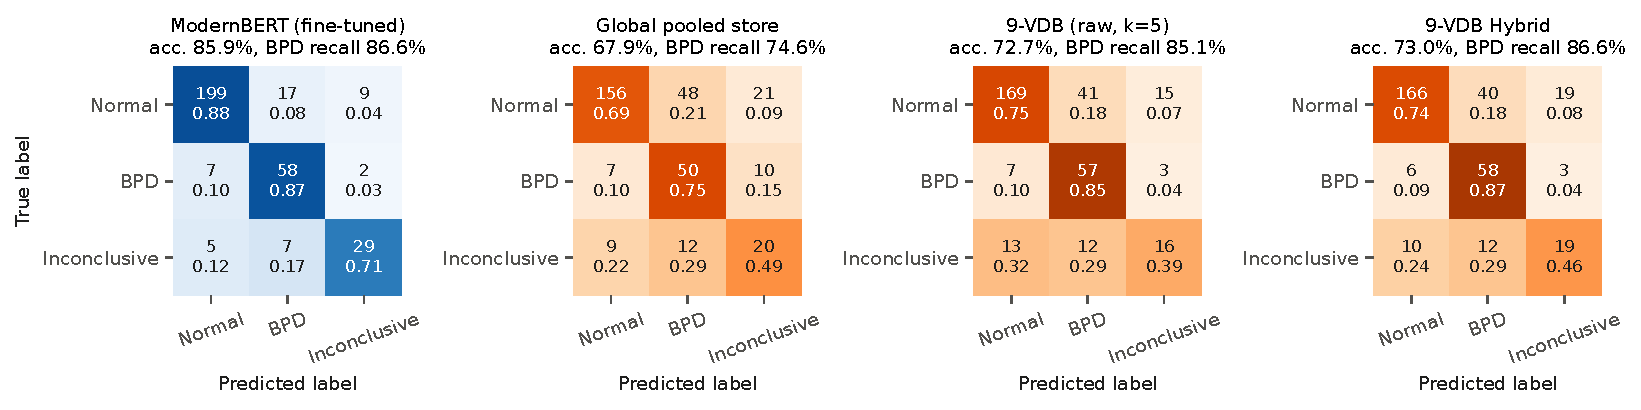
\includegraphics[width=\textwidth]{figures/generated/head_to_head_confusion.pdf}
\caption{Test confusion matrices of the best fine-tuned model (blue, seed 42) and three retrieval
configurations (orange).}
\label{fig:h2h}
\end{figure}

\begin{figure}[H]
\centering
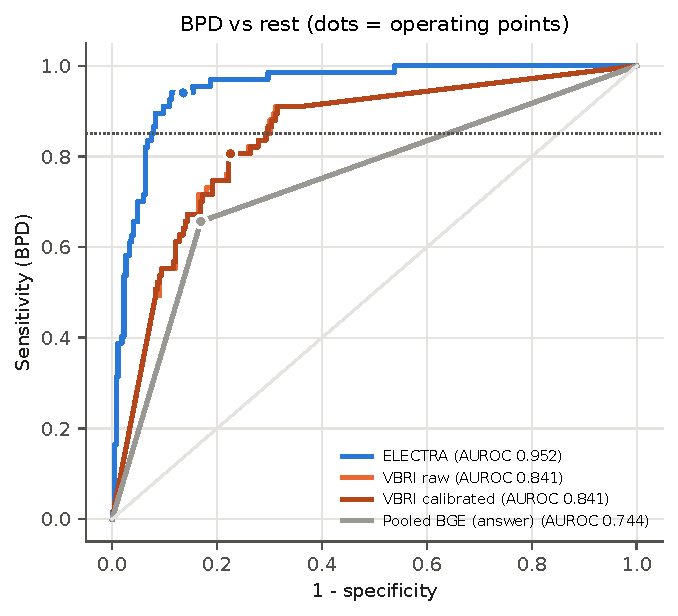
\includegraphics[width=0.55\textwidth]{figures/generated/roc_bpd.pdf}
\caption{ROC curves for BPD against the other two classes. The pooled baseline uses $k=1$, so its
curve has a single operating point.}
\label{fig:roc}
\end{figure}

\subsection{What fine-tuning costs and what semantic search saves}

Table~\ref{tab:cost} and Figure~\ref{fig:cost} answer RQ2.

\begin{table}[H]
\centering
\caption{Computational cost, measured on the same machine. Training time is the mean over three
seeds. Latency is the time per answer from text to prediction. Storage is what must be kept for this
task only; the shared \vbri{} encoder (about 438\,MB) is not counted.}
\label{tab:cost}
\small
\setlength{\tabcolsep}{4pt}
\resizebox{\textwidth}{!}{%
\begin{tabular}{@{}lcccccc@{}}
\toprule
\textbf{Model} & \textbf{Gradient updates} & \textbf{Train / index (s)} & \textbf{GPU bs 1 (ms)} & \textbf{GPU bs 32 (ms/ans.)} & \textbf{CPU bs 1 (ms)} & \textbf{Storage (MB)} \\
\midrule
ELECTRA & Yes & 275 $\pm$ 20 & 8.02 & 5.55 & 94.95 & 438.0 \\
BERT & Yes & 284 $\pm$ 35 & 8.62 & 5.73 & 93.69 & 438.0 \\
DistilBERT & Yes & 116 $\pm$ 9 & 4.55 & 2.90 & 46.82 & 267.8 \\
RoBERTa & Yes & 211 $\pm$ 14 & 8.26 & 5.49 & 94.90 & 498.6 \\
XLNet & Yes & 509 $\pm$ 72 & 16.10 & 8.14 & 131.31 & 469.3 \\
DeBERTa & Yes & 796 $\pm$ 130 & 23.98 & 7.58 & 179.49 & 737.7 \\
ModernBERT & Yes & 277 $\pm$ 39 & 24.57 & 8.82 & 119.81 & 598.4 \\
\midrule
\textbf{VBRI} & \textbf{No} & 9.6 & 10.09 & 2.27 & 68.94 & 12.5 \\
\bottomrule
\end{tabular}
}
\end{table}

\begin{figure}[H]
\centering
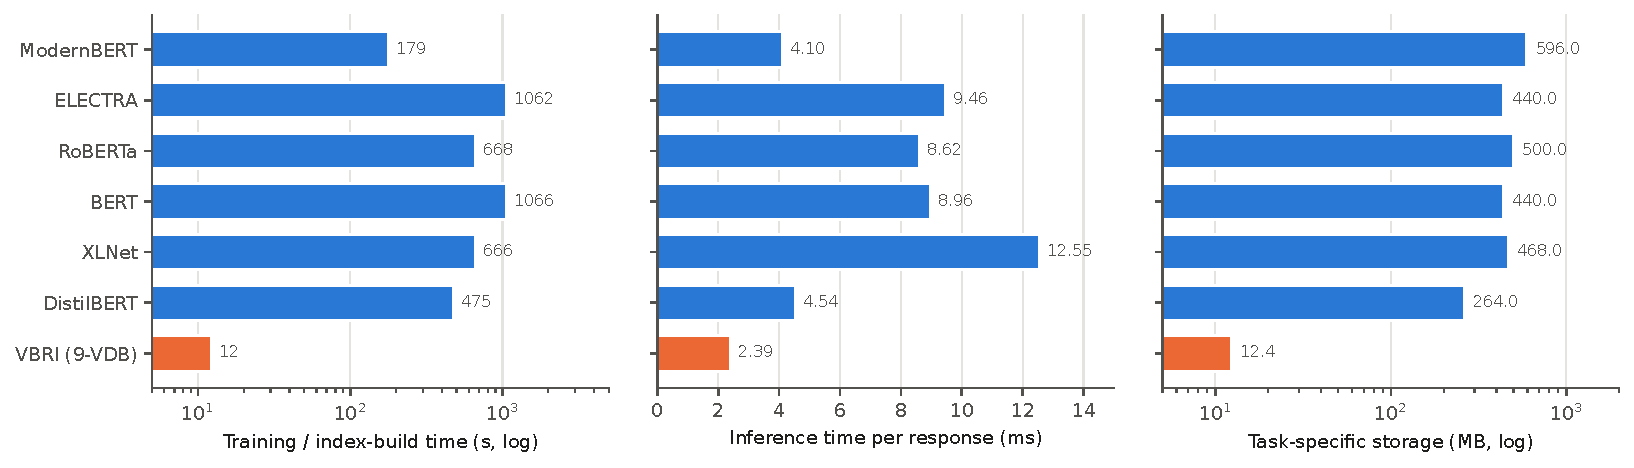
\includegraphics[width=\textwidth]{figures/generated/cost_comparison.pdf}
\caption{Training or index-build time, GPU and CPU latency with batch size 1, and task-specific
storage. The first and last panels use logarithmic scales.}
\label{fig:cost}
\end{figure}

The biggest saving is in \emph{building} the classifier. Fine-tuning took 116 to 796 seconds per run
on a GPU, and every change of data or labels needs a new run. \vbri{} needs one pass of the frozen
encoder over 4,050 answers, which took 9.6 seconds. This is 12 times faster than the quickest
fine-tuned model (DistilBERT) and 29 times faster than ELECTRA. When clinicians label new answers, we
insert rows. We do not retrain.

The task-specific \emph{storage} is 12.5\,MB, 21 to 59 times smaller than a fine-tuned model. A second
screening task needs a second small index, not a second copy of a large model. For a single task,
however, the encoder must also be on the device, so the total footprint is about the same as one
BERT-sized model.

At \emph{inference} the picture is mixed. With batch size 1 on the GPU, \vbri{} needs 10.1\,ms per
answer: slower than DistilBERT, ELECTRA, BERT and RoBERTa (4.6 to 8.6\,ms), and faster than XLNet,
DeBERTa-v3 and ModernBERT (16.1 to 24.6\,ms). With batch size 32 it was the fastest (2.3\,ms). On the
CPU it needed 68.9\,ms, faster than all fine-tuned models except DistilBERT (46.8\,ms). Almost all of
the \vbri{} time is spent encoding the query; the search takes about 0.1\,ms. Latencies changed by up
to about 30\% between sessions, so small differences should not be over-read.

\subsection{Per-criterion behaviour}

Table~\ref{tab:per_criterion} and Figure~\ref{fig:vdb_cm} break the \vbri{} result down by question.
\vbri{} is more accurate than the pooled index at the same $k$ on seven of the nine criteria and
less accurate on two (Q2 and Q7). The mean gain is 3.3 points and is not statistically significant
over nine criteria (paired $t$-test $p=0.12$, Wilcoxon $p=0.16$). The largest gains are for
abandonment (Q1, $+$10.8 points) and suicidal and self-harm behaviour (Q5, $+$8.1). Chronic emptiness
(Q7) loses 8.1 points. Each criterion has only 37 test answers, so one answer changes accuracy by 2.7
points.

\begin{table}[H]
\centering
\caption{Per-criterion comparison of the pooled index and \vbri{} raw ($k=3$ for both). Values in \%.}
\label{tab:per_criterion}
\scriptsize
\setlength{\tabcolsep}{3pt}
\resizebox{\textwidth}{!}{%
\begin{tabular}{@{}clcccccccc@{}}
\toprule
\textbf{Q} & \textbf{Criterion} & \textbf{N} & \textbf{Contam.} & \textbf{Pooled acc.} & \textbf{VBRI acc.} & \textbf{$\Delta$} & \textbf{Pooled BPD F1} & \textbf{VBRI BPD F1} & \textbf{$\Delta$} \\
\midrule
Q1 & Abandonment avoidance & 37 & 43.2 & 70.3 & 81.1 & +10.8 & 64.0 & 78.6 & +14.6 \\
Q2 & Unstable relationships & 37 & 37.8 & 62.2 & 59.5 & -2.7 & 42.1 & 45.5 & +3.3 \\
Q3 & Identity disturbance & 37 & 36.0 & 56.8 & 62.2 & +5.4 & 21.1 & 30.0 & +8.9 \\
Q4 & Impulsive behaviours & 37 & 34.2 & 78.4 & 83.8 & +5.4 & 44.4 & 44.4 & +0.0 \\
Q5 & Suicidal / self-harm & 37 & 41.4 & 83.8 & 91.9 & +8.1 & 33.3 & 40.0 & +6.7 \\
Q6 & Affective instability & 37 & 35.1 & 54.1 & 59.5 & +5.4 & 66.7 & 69.2 & +2.6 \\
Q7 & Chronic emptiness & 37 & 36.9 & 56.8 & 48.6 & -8.1 & 58.3 & 51.9 & -6.5 \\
Q8 & Inappropriate anger & 37 & 19.8 & 73.0 & 75.7 & +2.7 & 64.0 & 72.0 & +8.0 \\
Q9 & Paranoia / dissociation & 37 & 36.0 & 70.3 & 73.0 & +2.7 & 70.0 & 70.0 & +0.0 \\
\bottomrule
\end{tabular}
}
\end{table}

\begin{figure}[H]
\centering
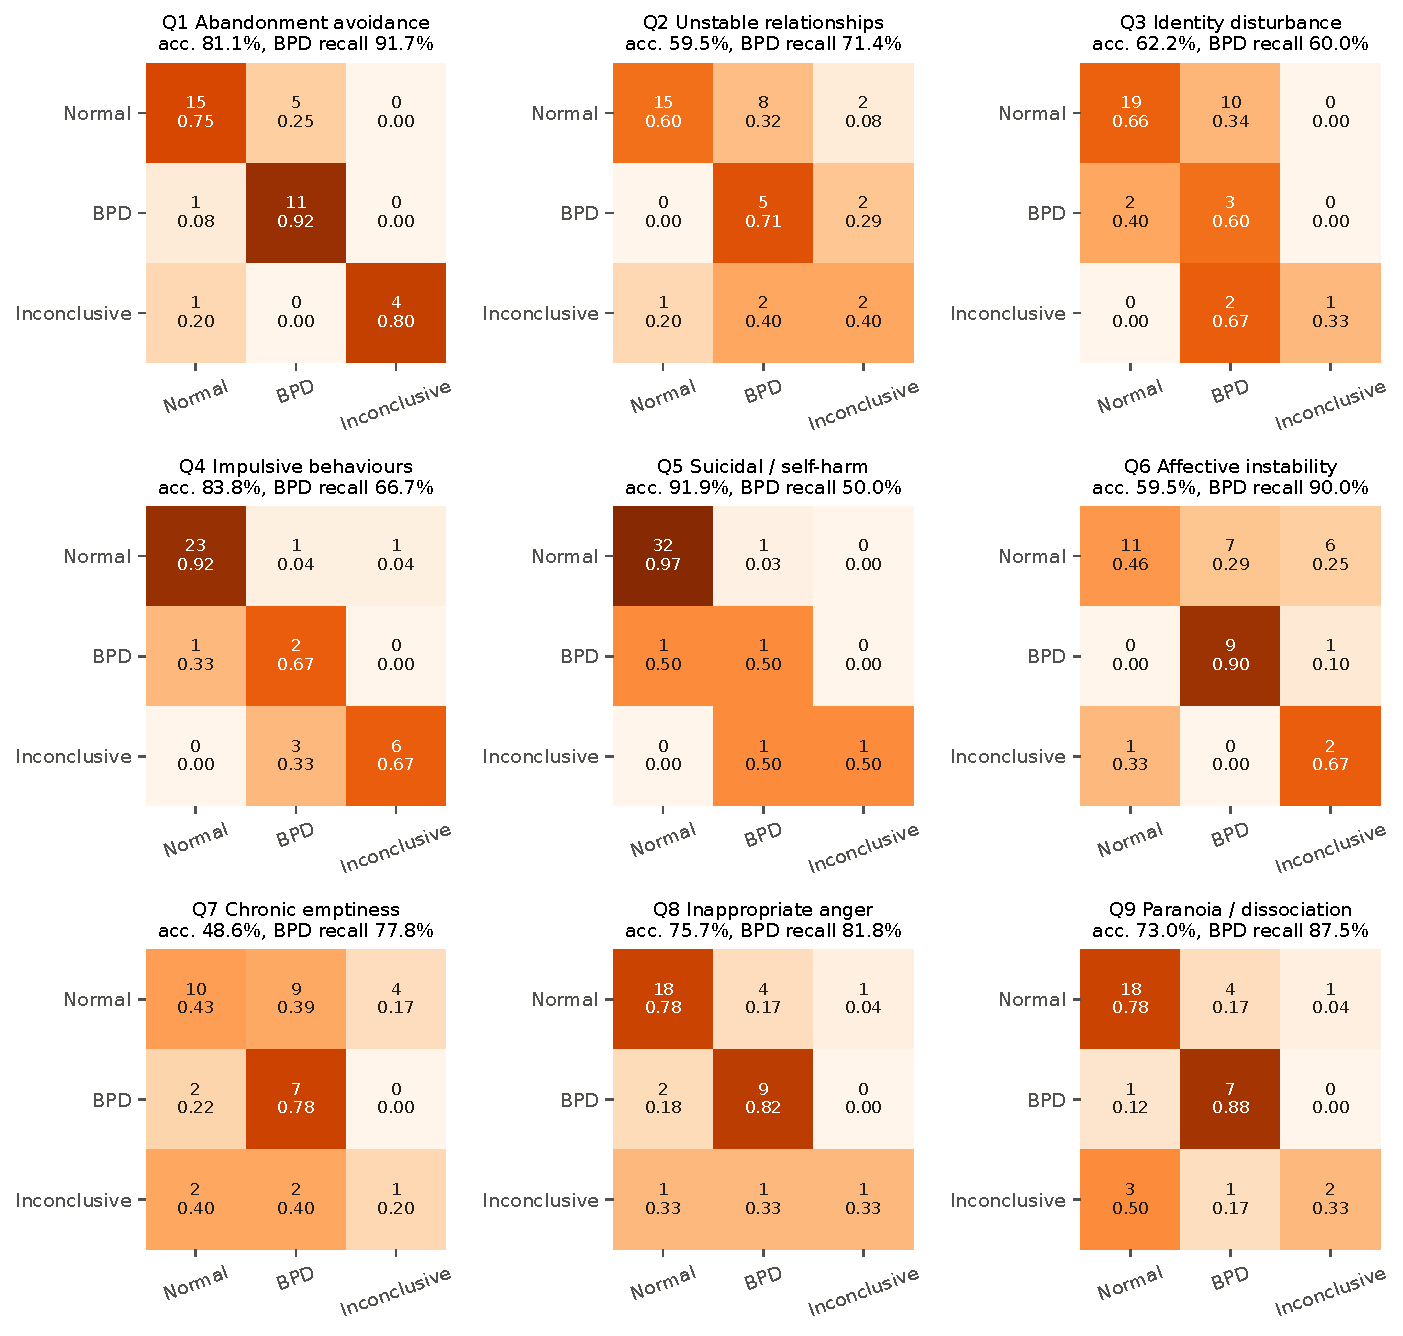
\includegraphics[width=\textwidth]{figures/generated/vdb_confusion_per_criterion.pdf}
\caption{\vbri{} confusion matrices for each of the nine \dsmv{} criteria (test set, 37 answers
each).}
\label{fig:vdb_cm}
\end{figure}

\begin{figure}[H]
\centering
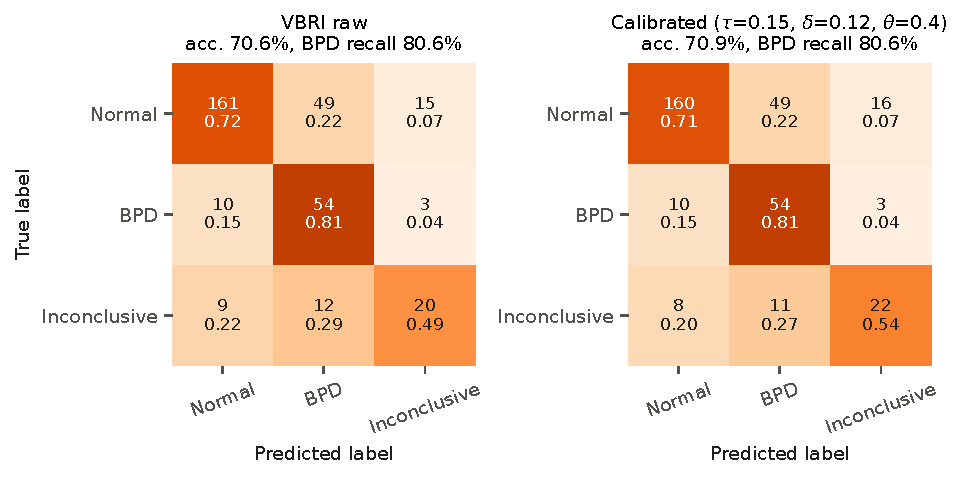
\includegraphics[width=0.75\textwidth]{figures/generated/calibration_before_after.pdf}
\caption{\vbri{} confusion matrix before (left) and after (right) calibration.}
\label{fig:calib}
\end{figure}

\subsection{Explainability: every decision comes with its evidence}

\vbri{} classifies by retrieval. So each prediction can be shown with the stored answers that
produced it. Table~\ref{tab:vignettes} gives four test cases, including one error. The retrieved
answers show what the decision rests on, and also when the evidence is weak or split. A fine-tuned
model can only give explanations after the fact. For \vbri{}, the explanation is the evidence that
was actually used.

\begin{table}[H]
\centering
\caption{Test cases with the retrieved neighbours (similarity in brackets).}
\label{tab:vignettes}
\scriptsize
\setlength{\tabcolsep}{4pt}
\resizebox{\textwidth}{!}{%
\begin{tabular}{@{}p{2.2cm}p{5.2cm}p{1.6cm}p{2.2cm}p{4.4cm}@{}}
\toprule
\textbf{Case} & \textbf{Answer (excerpt)} & \textbf{True} & \textbf{Predictions} & \textbf{Retrieved neighbours (VBRI)} \\
\midrule
Pooled index retrieves the wrong criterion (Q9) & ``I cannot control myself\ldots'' & Inconclusive & Pooled: Normal (100\% contam.)\newline VBRI: Inconclusive\newline Calibrated: Inconclusive & Inconclusive (0.67); Normal (0.67); BPD (0.67) \\
Uncertainty margin flags an ambiguous answer (Q7) & ``i do not think anything important is missing in my life\ldots'' & Inconclusive & Pooled: BPD (0\% contam.)\newline VBRI: BPD\newline Calibrated: Inconclusive & Normal (0.84); BPD (0.76); BPD (0.76) \\
Clear BPD-indicative answer (Q1) & ``Yes I felt the need to prevent someone leaving me emotionallly\ldots'' & BPD & Pooled: BPD (0\% contam.)\newline VBRI: BPD\newline Calibrated: BPD & BPD (0.93); BPD (0.88); BPD (0.88) \\
Error: negated statement read as BPD (Q9) & ``i never trust people... i always think, they are good for some reason until they have what they want. I have found that to be true most of the times\ldots'' & Normal & Pooled: Normal (67\% contam.)\newline VBRI: BPD\newline Calibrated: BPD & BPD (0.81); BPD (0.80); BPD (0.80) \\
\bottomrule
\end{tabular}
}
\end{table}

\subsection{Binary screening and participant-level agreement}

In practice, a screening tool often answers one question: should this person be referred? To test
this, we treat BPD as positive and the other two labels as negative (Table~\ref{tab:screening}).

\begin{table}[H]
\centering
\caption{Binary screening view (BPD vs.\ not BPD) on the test set ($N=333$, 67 positive). Values in
\%, except AUROC.}
\label{tab:screening}
\small
\resizebox{\textwidth}{!}{%
\begin{tabular}{@{}lcccccc@{}}
\toprule
\textbf{Model} & \textbf{Accuracy} & \textbf{Sensitivity} & \textbf{Specificity} & \textbf{PPV} & \textbf{NPV} & \textbf{AUROC} \\
\midrule
ELECTRA (fine-tuned, 3 seeds) & 88.69 $\pm$ 0.76 & 85.07 $\pm$ 7.76 & 89.60 $\pm$ 2.77 & 67.68 $\pm$ 3.75 & 96.04 $\pm$ 1.95 & 0.945 $\pm$ 0.007 \\
VBRI raw & 77.78 & 80.60 & 77.07 & 46.96 & 94.04 & 0.841 \\
VBRI calibrated & 78.08 & 80.60 & 77.44 & 47.37 & 94.06 & 0.841 \\
VBRI hybrid & 78.38 & 82.09 & 77.44 & 47.83 & 94.50 & -- \\
Pooled BGE (answer) & 79.58 & 65.67 & 83.08 & 49.44 & 90.57 & 0.744 \\
\bottomrule
\end{tabular}
}
\end{table}

\vbri{} raw has a negative predictive value of 94.04\% (ELECTRA: 96.04\%), so an answer that it
clears is usually not BPD. Its positive predictive value is 46.96\% (ELECTRA: 67.68\%): about half of
its positive flags are true BPD answers. This may be acceptable for a first-line screen in which a
clinician reviews every positive. It is not enough for a stand-alone decision.

We also checked participant-level agreement. There are 221 test participants, each with one to five
test answers. For each participant we counted the answers labelled BPD (Figure~\ref{fig:patient_level}).
ELECTRA agrees best with the expert count (mean absolute error 0.172, Pearson $r=0.77$). \vbri{} raw
has a higher correlation than the pooled index ($r=0.55$ vs.\ $0.48$) but a larger error (0.326 vs.\
0.290), because it flags more answers. No participant has more than two BPD-labelled answers in the
test split. So the \dsmv{} rule of five or more criteria cannot be tested here.

\begin{figure}[H]
\centering
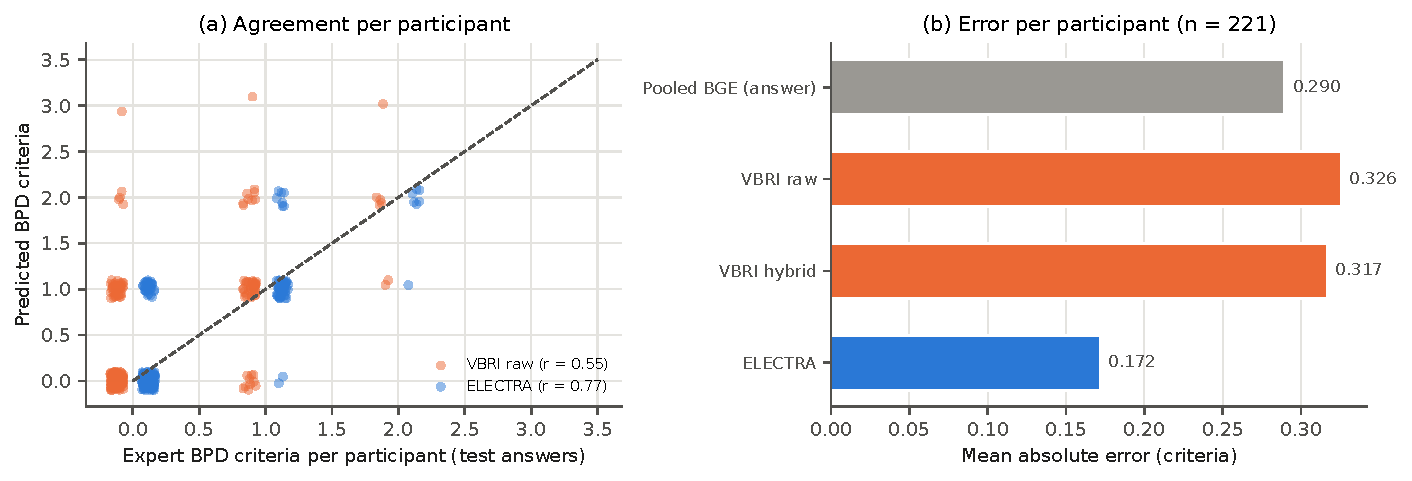
\includegraphics[width=\textwidth]{figures/generated/patient_level_agreement.pdf}
\caption{Participant-level agreement between predicted and expert-labelled BPD answer counts (221
test participants).}
\label{fig:patient_level}
\end{figure}

% =============================================================================
% 6. DISCUSSION
% =============================================================================
\section{Discussion}\label{sec:discussion}

\paragraph{So, do we need to fine-tune?}
For the best classifier on this data, yes. A fine-tuned encoder is about 13 points more accurate than
semantic search, raises far fewer false alarms and separates the three classes better. Its training
cost on a GPU is also modest here: 2 to 13 minutes. Semantic search makes sense under narrower
conditions: when there is no GPU for training, when labelled data change often, when one encoder
should serve several tasks, or when a clinician needs to see the evidence behind a decision. Under
these conditions, \vbri{} offers BPD sensitivity inside the range of fine-tuned models at a small
building and storage cost. It does not replace fine-tuning.

\paragraph{The index structure matters, within limits.}
A pooled index treats nine criteria as one problem, and about a third of its evidence comes from the
wrong question. Isolating the criteria removes this and finds more BPD answers on both the validation
and the test set. It did not clearly improve overall accuracy or macro F1. The recipe is still worth
considering for structured instruments with known item boundaries, such as psychiatric
questionnaires and triage forms, when sensitivity is the priority.

\paragraph{Relation to LLMs.}
We did not run generative LLMs, so our results say nothing direct about them. Other studies report
that prompted LLMs often do not beat fine-tuned encoders on classification~\cite{bucher2024finetuned,edwards2024icl},
and that they raise cost and privacy concerns for clinical text~\cite{guo2024llmreview}. Comparing
them with \vbri{} on this data is an important next step.

\paragraph{Limitations.}
This study has several limits. They should be addressed before any clinical use.
\begin{itemize}[leftmargin=*,itemsep=2pt]
  \item \emph{Earlier development choices.} Retrieval settings were chosen on the validation set. The
        BGE encoder and the C-SSRS rule were chosen in earlier development, where test results had
        been seen. They should be confirmed on new data.
  \item \emph{Negation and short disclosures.} \vbri{} raw made 98 errors. Of these, 49 were Normal
        answers labelled BPD, and 27 of those contain an explicit negation (``never'', ``not'',
        ``nothing''). Sentence embeddings often place negated statements close to affirmative
        ones~\cite{chiang2023heros,cao2025negation}.
  \item \emph{One dataset, one language, one domain.} \bpdqac{} is a single English dataset with 362
        mostly student participants. The test set has 333 answers, 67 of them BPD, so one answer is
        1.5 points of sensitivity. Splits are at answer level, so one participant can have answers in
        both the training and test sets, for different questions.
  \item \emph{Augmented training text.} Of the 4,050 training answers, 1,800 are augmented, about two
        thirds of the BPD and Inconclusive classes. This affects both paradigms.
  \item \emph{Training details.} DeBERTa-v3 used fp32 and the other models fp16. The software version
        used (transformers 5.0.0) reported mismatched layer-normalisation parameter names when some
        models reloaded their best checkpoint. For those models, the layer-normalisation values may
        not come from the best epoch.
  \item \emph{Hardware.} All timings come from one cloud machine (Tesla T4 GPU and its CPU). We did
        not test mobile or low-power devices.
\end{itemize}

% =============================================================================
% 7. CONCLUSION
% =============================================================================
\section{Conclusion}\label{sec:conclusion}

This paper asked a simple question. Must a clinical text classifier be fine-tuned, or can semantic
search over a frozen embedding model do the job? On structured BPD interview answers, fine-tuned
encoders are clearly better: ELECTRA reaches 83.88\% accuracy against 70.57\% for our training-free
classifier \vbri{}. \vbri{} still finds 80.60\% of BPD answers, inside the range of the fine-tuned
means. It replaces GPU training with a 9.6-second indexing step, adds only a 12.5\,MB index per task
to a shared encoder, and shows the evidence behind every decision. Isolating the criteria and
balancing each database raise BPD sensitivity compared with a pooled index, but not overall accuracy
by a clear margin. Semantic search is therefore a practical option for transparent,
sensitivity-focused screening where training is difficult. It is not a general replacement for
fine-tuning.

\section*{Data Availability}

The \bpdqac{} dataset is available at \textless{}repository link\textgreater{} as a CSV file. It
contains unique identifiers, question texts, participant responses, expert-annotated labels and
binary indicators for Criteria B through F. The experiment code, which produces the numbers, tables
and result figures in this paper, is provided as supplementary material.

\printbibliography

\end{document}
